\documentclass[a4paper,10pt]{report}

% language settings
\usepackage[utf8]{inputenc}
\usepackage{polski}
\usepackage[polish]{babel}

% listings
\usepackage{listings}
\lstset{
  language=Java,
  numbers=left,
  numbersep=5pt,
  breaklines=true,
  basicstyle=\footnotesize\ttfamily,
  numberstyle=\footnotesize,
  showspaces=false,
  showstringspaces=false
}

% graphics
\usepackage{graphicx}

% other settings
\usepackage{setspace}
\title{Apache Lucene jako przykład wykorzystania architektury kodekowej w implementacji silnika wyszukiwania tekstowego}
\author{Aleksandra Woźniak}

\begin{document}
\begin{titlepage}

\begin{spacing}{2}

\begin{center}
 \vspace*{5cm}
 {\LARGE Apache Lucene jako przykład wykorzystania architektury kodekowej w implementacji silnika wyszukiwania tekstowego}
 \\[0.75cm]
 {\Large Aleksandra Woźniak}
 \\[0.3cm]
 {\large 24 października 2013}
 \\[2.5cm]
 {\large Praca magisterska napisana pod kierunkiem dra Piotra Wieczorka
 \\[4cm]
 Instytut Informatyki\\
 Wydział Matematyki i Informatyki \\
 Uniwersytetu Wrocławskiego}

\end{center}

\end{spacing}

\end{titlepage}
\begin{abstract}
 Praca stanowi przedstawienie biblioteki Apache Lucene -- popularnego silnika wyszukiwania tekstowego, napisanego w języku Java i dostępnego na licencji open source. W pracy poruszone są następujące zagadnienia: funkcjonalności biblioteki (indeksowanie dokumentów, wyszukiwanie, operacje na wynikach wyszukiwania, możliwości rozszerzenia i podmiany standardowych mechanizmów analizy tekstu lub modelu oceny zgodności dokumentu z zapytaniem), jej architektura (ze szczególnym naciskiem na opis architektury kodekowej) oraz zaimplementowany algorytm łączenia list postingowych (wraz z propozycją jego modyfikacji).
\end{abstract}

\chapter{Wprowadzenie}

W ciągu ostatnich kilkudziesięciu lat obserwujemy zjawisko zwane ,,eksplozją danych'': ilość informacji zgromadzonych przez ludzkość rośnie eksponencjalnie. Dostępność informacji nie byłaby jednak do niczego przydatna -- bez możliwości efektywnego ich przeszukiwania. Dodatkowo, większość danych, które codziennie produkujemy nie posiada wyraźnej struktury.  Wyszukiwanie interesujących fragmentów w takich zbiorach nie jest więc problemem trywialnym. Dlategoteż tak ważne stało się tworzenie narzędzi to ułatwiających -- wyszukiwarek. 

Celem niniejszej pracy jest przedstawienie biblioteki Apache Lucene pozwalającej tworzyć wyszukiwarki dokumentów tekstowych. W kolejnych rozdziałach opisane zostaną: funkcjonalności oferowane przez Lucene, jej architektura oraz przytoczone zostaną przykłady jej wykorzystania.

\section{Apache Lucene}

Lucene jest jedną z najpopularniejszych bibliotek wyszukiwania tekstowego. Jest napisana w całości w języku Java i udostępniona jest na licencji open source.

Apache Lucene skupia w sobie cztery główne podprojekty: 
\begin{itemize}
 \item \emph{Lucene Core}, będący faktyczną implementacją silnika wyszukiwania. Na opisie tego właśnie podprojektu skupimy się w tej pracy. W dalszej części tekstu termin ,,Lucene'' będzie odnosił się do Lucene Core.
 \item \emph{Solr} jest implementacją serwera wyszukiwania, wykorzystującą Lucene Core jako silnik. Solr, poza wyszukiwaniem tekstowym, udostępnia takie funkcjonalności jak integracja z bazą danych, operowanie na popularnych formatach dokumentów (Word, PDF) czy wyszukiwanie po współrzędnych geograficznych.
 \item \emph{Open Relevance Project} dostarcza narzędzi do testowania trafności wyników wyszukiwania.
 \item \emph{PyLucene} jest rozszerzeniem Pythona pozwalającym na korzystanie z możliwości Lucene.
\end{itemize}

Dokumentacja Lucene Core wymienia m.in. następujące cechy charakterystyczne biblioteki:
\begin{itemize}
 \item szybkie, skalowalne indeksowanie dokumentów -- z możliwościami indeksowania inkrementalnego wykazującego się podobnymi właściwościami,
 \item rozmiar indeksu nie przekraczający 20-30\% rozmiaru pierwotnych dokumentów,
 \item wyszukiwanie połączone z sortowaniem wyników zgodnie z malejącą trafnością dopasowania do zapytania,
 \item dostępność wielu rodzajów zapytań,
 \item zdefiniowane przez użytkownika sortowanie wyników,
 \item możliwość konfiguracji formatu plików indeksu (architektura oparta o kodeki).
\end{itemize}

Lucene Core, pomimo, że napisana w Javie, może być wykorzystana także w innych językach. Umożliwiają to liczne projekty towarzyszące, m.in. CLucene (implementacja w C++), Lucene.NET (portowanie biblioteki na platformę .NET) i LuceneKit (implementacja w języku Objective-C wraz ze wsparciem dla natywnej dla środowiska MacOS X biblioteki Cocoa i jej open source'owej implementacji GNUstep). Wszystkie implementacje Lucene gwarantują kompatybilność utworzonych przez nie indeksów.

\section{Przykład wykorzystania Lucene}

Poniżej zamieszczony jest prosty program wykorzystujący Lucene. Indeksuje on dokumenty z zadanego katalogu i pozwala na wyszukiwanie tych z nich, które zawierają podane przez użytkownika słowo kluczowe. Bazę dokumentów stanowi zbiór pięciu anglojęzycznych książek, pobranych ze strony Projektu Gutenberg \cite{gutenberg}.

Oto przykładowy wynik uruchomienia programu:
\begin{lstlisting}[escapeinside={@}{@}]
@\label{result-1:enter}@Enter a single word query:
thing
@\label{result-1:query}@Documents matching the query: contents:thing
@\label{result-1:begin}@Lewis Carroll - Alice's Adventures in Wonderland.txt
James M. Barrie - Peter Pan.txt
Emily Bronte - Wuthering Heights.txt
Arthur Conan Doyle - The Adventures of Sherlock Holmes.txt
@\label{result-1:end}@Jane Austen - Pride and Prejudice.txt
\end{lstlisting}

Po zaindeksowaniu dokumentów program pyta użytkownika o zapytanie, po którym ma odbywać się wyszukiwanie (linia \ref{result-1:enter}). Gdy użytkownik wprowadzi słowo kluczowe, następuje proces wyszukiwania. Program wypisuje zapytanie (linia \ref{result-1:query}) a następnie -- tytuły pasujących dokumentów (linie \ref{result-1:begin}-\ref{result-1:end}). Zauważmy, że zapytanie składa się z dwóch elementów: pola, po ktorym ma odbywać się wyszukiwanie oraz słowa kluczowego, oddzielonych dwukropkiem.

Zapytanie użyte w powyższym przykładzie jest jednym z najpopularniejszych słów języka angielskiego -- nie dziwi więc fakt, że w wyniku otrzymaliśmy wszystkie dokumenty. Jeśli użyjemy mniej popularnego słowa, lista pasujących dokumentów będzie krótsza.

\begin{lstlisting}[escapeinside={@}{@}]
Enter a single word query:
suspect
Documents matching the query: contents:suspect
Jane Austen - Pride and Prejudice.txt
Emily Bronte - Wuthering Heights.txt
Arthur Conan Doyle - The Adventures of Sherlock Holmes.txt
\end{lstlisting}

\subsection{Struktura programu}

Zamieszczona poniżej metoda \texttt{main()} ilustruje przebieg programu.

\begin{lstlisting}[escapeinside={@}{@}]
/**
 * Maximum number of results returned by IndexSearcher instance.
 */
@\label{main:MAX_DOCS}@private static final int MAX_DOCS = 10;

/**
 * Relative path to a folder containing documents for indexing.
 */
private static final String CORPUS_FOLDER_PATH = "../books";

/**
 * An index directory.
 */
@\label{main:directory}@private static final Directory directory = new RAMDirectory();

public static void main(String[] args) throws IOException {
  @\label{main:createIndex}@createIndex(directory, CORPUS_FOLDER_PATH);
  @\label{main:obtainQuery}@Query query = obtainQuery();
  @\label{main:createIndexSearcher}@IndexSearcher searcher = createIndexSearcher(directory);
  // Perform search.
  @\label{main:search}@TopDocs topDocs = searcher.search(query, MAX_DOCS);
  @\label{main:printResults}@printResults(query, searcher, topDocs);
}
\end{lstlisting}

W linii \ref{main:createIndex} tworzony jest indeks. Metoda \texttt{createIndex()} jako parametry przyjmuje obiekt typu \texttt{Directory} oraz ścieżkę do folderu zawierającego dokumenty do zaindeksowania. \texttt{Directory} jest interfejsem reprezentującym katalog zawierający pliki indeksu. W opisywanym przykładzie posługujemy się indeksem trzymanym w pamięci podręcznej, stąd korzystamy z implementacji \texttt{RAMDirectory} (linia \ref{main:directory}).

Następnie, w linii \ref{main:obtainQuery} tworzymy obiekt typu \texttt{Query}, reprezentujący zapytanie. Klasą odpowiedzialną za przeszukiwanie indeksu jest \texttt{IndexSearcher} -- tworzony w linii \ref{main:createIndexSearcher}. Faktyczne wyszukiwanie odbywa się poprzez wykonanie polecenia \texttt{searcher.search(query, MAX\_DOCS)} w linii \ref{main:search} (\texttt{MAX\_DOCS} -- linia \ref{main:MAX_DOCS} -- jest maksymalną liczbą wyników, które może zwrócić proces wyszukiwania). Program kończy się wypisaniem wyników w linii \ref{main:printResults}.

\subsection{Tworzenie indeksu}

Metoda \texttt{createIndex()} ilustruje proces tworzenia indeksu: na początku tworzony jest obiekt typu \texttt{IndexWriter} (linia \ref{createIndex:indexWriter}) oraz lista dokumentów (linia \ref{createIndex:documents}). Po dodaniu dokumentów do zapisu (linia \ref{createIndex:add}) następuje commit oraz zamknięcie obiektu \texttt{indexWriter} (linie \ref{createIndex:commit} -- \ref{createIndex:close}).

\begin{lstlisting}[label=createIndex,escapeinside={@}{@}]
private static void createIndex(Directory directory, String path) throws IOException {
  @\label{createIndex:indexWriter}@IndexWriter indexWriter = createIndexWriter(directory);
  @\label{createIndex:documents}@List<Document> documents = createDocuments(path);
  @\label{createIndex:add}@indexWriter.addDocuments(documents);
  @\label{createIndex:commit}@indexWriter.commit();
  @\label{createIndex:close}@indexWriter.close();
}

private static IndexWriter createIndexWriter(Directory directory) throws IOException {
  @\label{indexWriter:config}@IndexWriterConfig config = new IndexWriterConfig(Version.LUCENE_44, new StandardAnalyzer(Version.LUCENE_44));
  return new IndexWriter(directory, config);
}
\end{lstlisting}

\texttt{IndexWriter} jest klasą odpowiedzialną za zapis struktur indeksu do wskazanego katalogu. Poza obiektem typu \texttt{Directory}, \texttt{IndexWriter} przyjmuje w konstruktorze obiekt konfiguracji: \texttt{IndexWriterConfig} (linia \ref{indexWriter:config}), który z kolei potrzebuje instancji typu \texttt{Analyzer} (wykorzystaną tutaj implementacją jest \texttt{StandardAnalyzer}). \texttt{Analyzer} definiuje sposób ekstrakcji termów z dokumentu.

Dokumenty tworzone są na podstawie plików zawartych we wskazanym folderze.

\begin{lstlisting}
private static List<Document> createDocuments(String path) throws IOException {
  List<Document> documents = new ArrayList<>();
  File documentsFolder = new File(path);
  if (!documentsFolder.isDirectory()) {
    throw new IOException("Specified path does not point to a directory.");
  }
  File[] files = documentsFolder.listFiles();
  for (File file : files) {
    if (!file.isDirectory() && !file.isHidden() && file.exists() && file.canRead()) {
      Document document = createDocument(file);
      documents.add(document);
    }
  }
  return documents;
}
\end{lstlisting}

Pojedynczy dokument (\texttt{Document}) jest zbiorem pól. Każde pole ma określony typ (wyspecyfikowany przez implementację abstrakcyjnej klasy \texttt{Field}), nazwę (podawaną jako pierwszy parametr konstruktora) oraz zawartość. Opcjonalnie zawartość ta może być zapisana w plikach indeksu -- aby można było później ją zwrócić w wyniku wyszukiwania. Przykład takiego pola znajduje się w linii \ref{createDocument:store} poniższego listingu: podczas tworzenia pola \texttt{filename} jako trzeci parametr konstruktora podane jest \texttt{Field.Store.YES} .

\begin{lstlisting}[label=createDocument,escapeinside={@}{@}]
/**
 * Field names.
 */
public static final String CONTENT_FIELD = "contents";
public static final String FILE_NAME_FIELD = "filename";

private static Document createDocument(File file) throws FileNotFoundException {
  Document document = new Document();
  document.add(new TextField(CONTENT_FIELD, new FileReader(file)));
  @\label{createDocument:store}@document.add(new StringField(FILE_NAME_FIELD, file.getName(), Field.Store.YES));
  return document;
}
\end{lstlisting}

\subsection{Tworzenie zapytania}

Zapytanie jest tworzone na podstawie wczytanego z linii poleceń tekstu. Korzystamy z klasy \texttt{TermQuery} implementującej abstrakcyjne \texttt{Query} -- reprezentującej zapytanie składające się z pojedynczego termu. Ponieważ w Lucene termy identyfikowane są przez parę \emph{pole:term}, posługujemy się także nazwą pola, w którym odbywać się będzie wyszukiwanie (linia \ref{obtainQuery:termQuery}).

\begin{lstlisting}[label=obtainQuery,escapeinside={@}{@}]
private static Query obtainQuery() {
  System.out.println("Enter a single word query:");
  Scanner scanner = new Scanner(System.in);
  String queryString = scanner.nextLine().trim();
  scanner.close();
  @\label{obtainQuery:termQuery}@return new TermQuery(new Term(CONTENT_FIELD, queryString));
}
\end{lstlisting}

\subsection{Wyszukiwanie}

Obiektem odpowiedzialnym za wykonywanie zapytań na indeksie jest \\ \texttt{IndexSearcher}. Sposób tworzenia go ilustruje poniższy listing.

\begin{lstlisting}
private static IndexSearcher createIndexSearcher(Directory directory) {
  IndexReader reader = null;
  try {
    reader = DirectoryReader.open(directory);
  } catch (IOException e) {
    e.printStackTrace();
  }
  return new IndexSearcher(reader);
}
\end{lstlisting}

\subsection{Wypisywanie wyników}

Metoda \texttt{search()} klasy \texttt{IndexSearcher} zwraca obiekt typu \texttt{TopDocs}, który m.in. zawiera listę najlepiej pasujących do zapytania dokumentów. Listing poniżej pokazuje sposób uzyskania i wykorzystania tej listy (dla każdego dokumentu obecnego w wyniku, program wypisuje na konsolę nazwę pliku odpowiadającemu temu dokumentowi).

\begin{lstlisting}
private static void printResults(Query query, IndexSearcher searcher, TopDocs topDocs) throws IOException {
  System.out.println("Documents matching the query: " + query);
  for (ScoreDoc scoreDoc : topDocs.scoreDocs) {
    Document document = searcher.doc(scoreDoc.doc);
    String documentTitle = document.get(FILE_NAME_FIELD);
    System.out.println(documentTitle);
  }
}
\end{lstlisting}

\chapter{Funkcjonalności Lucene}

W niniejszym rozdziale zostaną przedstawione główne funkcjonalności Lucene: indeksowanie oraz wyszukiwanie. Poruszone też będą bardziej zaawansowane zagadnienia, takie jak budowa własnego mechanizmu analizy tekstu czy miary oceny dopasowania dokumentu do zapytania. Poszczególne kwestie celowo opisane są skrótowo -- celem pracy jest bowiem opis architektury biblioteki, a nie jej możliwości. Funkcjonalności Lucene są tu wspomniane jedynie dla pełności opisu.

%-----------------------------------------------------
\section{Przygotowanie do indeksowania: analiza tekstu}

Lucene przechowuje dane w~strukturze zwanej \emph{indeksem odwróconym}. Zanim jednak indeksowany tekst trafi do tej struktury, musi przejść przez proces analizy. Indeks odwrócony budowany jest na bazie tzw. \emph{tokenów}, które możemy dla uproszczenia zdefiniować jako podstawowe formy słów poddawane indeksowaniu. Proces analizy polega, w~ogólności, na utworzeniu strumienia tokenów na podstawie zadanego tekstu. Może on obejmować takie operacje jak odfiltrowanie stop-words, sprowadzenie słowa do jego formy podstawowej (poprzez stemming lub przy użyciu analizy morfologicznej), czy wykrycie i~zaindeksowanie synonimów. 

Analiza tekstu jest problemem nietrywialnym. Od narzędzi ją wykonujących wymagamy, aby różnorodne formy tego samego słowa (jak liczba mnoga, odmiany fleksyjne) były sprowadzone do tej samej bazy, aby poprawnie rozróżniane były nazwy własne, numery, daty czy nazwiska. Oczywiście, istniejące obecnie rozwiązania nie spełniają tych wymagań w~stu procentach.

Analiza tekstu w~Lucene jest zazwyczaj wykonywana w~dwóch sytuacjach: podczas indeksowania nowego dokumentu oraz podczas parsowania zapytań. Dodatkowo, tekst pobrany z~indeksu może być niekiedy analizowany powtórnie (np. jeśli mają być w~nim zaznaczone wystąpienia wyszukiwanych słów).

W Lucene za analizę danych jest odpowiedzialna abstrakcyjna klasa \texttt{Analyzer} oraz jej nieabstrakcyjne rozszerzenia, wśród których najpopularniejszym jest \texttt{StandardAnalyzer}. Istnieje także możliwość utworzenia własnego narzędzia analizy tekstu. 

\subsection{Struktura Analyzera}

\texttt{Analyzer} jest abstrakcyjną klasą definiującą zarys algorytmu analizy tekstu. Lucene dostarcza kilku jej uniwersalnych implementacji, które dla większości zastosowań okazują się być wystarczające -- dlatego rzadko konieczne jest pisanie własnego \texttt{Analyzera}. Najczęściej wykorzystywaną implementacją jest \texttt{StandardAnalyzer}.

Algorytm analizy tekstu składa się z~trzech faz:
\begin{enumerate}
 \item \emph{pre-tokenizacji}: faza ta na wejściu oczekuje czystego tekstu, jej wyjściem jest również tekst. Polega na odfiltrowaniu niepożądanych znaków lub fragmentów tekstu (takich jak np. znaki interpunkcyjne czy znaczniki HTML). Implementowana jest przez jedną bądź wiele klas typu \texttt{CharFilter} (filtry mogą być łączone w~łańcuchy). Faza pre-tokenizacji jest opcjonalna -- wiele analizerów całkowicie ją pomija.
 \item \emph{tokenizacji}: wejściem dla algorytmu tokenizacji jest czysty tekst, wyjściem -- strumień obiektów typu \texttt{Token}. Tokenizacja (podział tekstu na tokeny) zazwyczaj odbywa się na podstawie białych znaków występujących w~tekście. Klasą odpowiedzialną za przeprowadzenie tej fazy jest \texttt{Tokenizer}.
 \item \emph{post-tokenizacji}: zarówno wejściem jak i~wyjściem tej fazy jest strumień \texttt{Tokenów}. W niej odbywają się takie operacje jak stemming, usunięcie stop-words czy wprowadzenie synonimów do strumienia. Post-tokenizacja odbywa się przy użyciu  jednej lub kilku klas implementujących abstrakcyjny \texttt{TokenFilter}. Podobnie, jak w~przypadku pre-tokenizacji, filtry można łączyć w~łańcuchy.
\end{enumerate}

Tworzenie własnego \texttt{Analyzera} polega na zaimplementowaniu (lub wykorzystaniu dostępnych) komponentów: (opcjonalnie) \texttt{CharFilterów}, \texttt{Tokenizera} oraz \texttt{TokenFilterów}. 

\subsection{Ekstrakcja treści ze złożonych dokumentów}

Jedyną formą danych akceptowaną przez Lucene jest czysty tekst. Lucene nie dostarcza żadnych narzędzi pozwalających na wyekstrahowanie tekstu z~dokumentów o rozbudowanej strukturze (np. w~formatach HTML, PDF, MS Word). Zatem odpowiedzialność parsowania złożonych dokumentów leży po stronie aplikacji wykorzystującej Lucene. 

%---------------------------------------------------
\section{Indeksowanie danych}

Aby zrozumieć, w~jaki sposób dane przechowywane są indeksie Lucene, wyjaśnimy na początku kilka pojęć:
\begin{itemize}
 \item \emph{Term} -- jest podstawową jednostka wyszukiwania i~indeksowania. Term jest ściśle związany z~polem, w~jakim występuje. Dlatego pojedynczy term utożsamiamy z~parą \emph{nazwa pola:słowo}.
 \item \emph{Pole} -- jest to zbiór termów, oznaczony identyfikującą go nazwą i~posiadający określony typ. Pole posiada też pewne parametry wskazujące, jak jego zawartość (lista należących do niego termów) powinna być traktowana podczas indeksowania i~wyszukiwania. Określa np. czy zawartość powinna być tokenizowania lub przechowywana w~indeksie. Wartości tych parametrów są na ogół zależne od wybranego typu pola.
 \item \emph{Dokument} -- jest zbiorem pól. Jest identyfikowany przez swój numer, unikalny w~obrębie segmentu. Dokumenty w~Lucene nie mają narzuconej, sztywnej struktury. Oznacza to, że w~obrębie jednego indeksu mogą występować dokumenty o całkowicie różnych zbiorach pól. 
\end{itemize}

Dokumenty dodawane do Lucene są przechowywane w~indeksie odwróconym, który mówiąc w~uproszczeniu, jest strukturą mapującą termy na listy numerów dokumentów zawierających dany term. Na pojedynczy indeks może składać się wiele \emph{segmentów}. Segment jest sam w~sobie w~pełni funkcjonalnym indeksem -- podział indeksu na mniejsze jednostki pozwala m.in. na zrównoleglenie procesu wyszukiwania.

\subsection{Typy pól}

Lucene pozwala na utworzenie pól następujących typów:
\begin{enumerate}
 \item pola tekstowe: \texttt{TextField} i~\texttt{StringField}. Pola obydwóch typów są indeksowane, różnica między nimi polega na tym, że \texttt{StringField} nie jest dzielone na tokeny -- cała jego zawartość traktowana jest jako pojedynczy token. Wobec tego nadaje się np. do przechowywania numerów identyfikacyjnych, nazwisk czy nazw państw. \texttt{TextField} jest polem indeksowanym i~analizowanym -- zazwyczaj występuje jako główne pole dokumentu, przechowujące większą część treści. Opcjonalnie, obydwa typy pól tekstowych mogą być przechowywane w~indeksie (\emph{stored fields}).
 \item pola numeryczne: \texttt{IntField}, \texttt{LongField}, \texttt{DoubleField}, \texttt{FloatField}. Pozwalają na indeksowanie wartości liczbowych oraz na późniejsze wyszukiwanie i~filtrowanie po zakresach wartości. Każde pole typu numerycznego jest indeksowane jako drzewo trie.
 \item pole ,,przechowywane'', \texttt{StoredField}: pole, którego pełna zawartość jest przechowywana w~indeksie i~może być odzyskana podczas wyszukiwania. Tego typu pole zazwyczaj stosuje się do zapisu takich informacji jak tytuł czy abstrakt dokumentu, jego zawartość nie jest jednak ograniczona do tekstu -- \texttt{StoredField} może także przechowywać liczby lub wartości binarne.
 \item pola typu DocValues: \texttt{NumericDocValuesField}, \texttt{BinaryDocValuesField}, \texttt{SortedDocValuesField}, \texttt{SortedSetDocValuesField} -- jest to nowy typ pola, wprowadzony w~wersji 4.0 Lucene. Zawartości pól typu DocValues nie są włączane do indeksu odwróconego -- a zatem nie można po nich wyszukiwać. Są natomiast przydatne podczas sortowania lub grupowania wyników wyszukiwania. W przeciwieństwie do indeksu odwróconego, DocValues zaimplementowane są jako struktura mapująca indeksy dokumentów na zadane wartości (typu zależnego od wybranej implementacji pola). DocValues istnieją niezależnie od głównego indeksu. Są jedynie optymalizującym dodatkiem do Lucene -- funkcje, do jakich są wykorzystywane mogłyby zostać spełnione przez pola innych typów, kosztem czasu wykonania. 
\end{enumerate}

%----------------------------------------------
\section{Operacje na indeksie}

Podstawowym elementem, na którym operujemy podczas indeksowania jest dokument. Jak zostało to pokazane w~pierwszym rozdziale, abstrakcją go opakowującą jest klasa \texttt{Document}. Dokumenty mogą być do indeksu dodawane, usuwane z~niego lub odświeżane w~indeksie.

\subsection{Dodawanie dokumentów}

Przykład dodawania dokumentów został zaprezentowany w~pierwszym rozdziale pracy. \texttt{Document}, tworzony na podstawie pól, jest zapisywany w~indeksie za pośrednictwem klasy \texttt{IndexWriter}.

\subsection{Usuwanie dokumentów}

Usuwanie dokumentów może odbyć się na jeden z~trzech sposobów: 
\begin{enumerate}
 \item usunięcie dokumentów zawierających określony term (lub zawierających co najmniej jeden z~podanego zbioru termów),
 \item usunięcie dokumentów pasujących do danego zapytania (lub pasujących do co najmniej jednego zapytania z~podanego zbioru),
 \item usunięcie wszystkich dokumentów z~indeksu.
\end{enumerate}

Wszystkie wymienione wyżej sposoby są realizowane przez klasę \texttt{IndexWriter} -- tę samą, która służy do dodawania dokumentów. Proces usuwania odbywa się następująco: początkowo dany dokument zostaje jedynie \emph{zaznaczony} jako usunięty. Fizycznie cały czas jest obecny w~indeksie odwróconym. Rozwiązanie to zastosowane jest ze względów optymalizacyjnych: wyszukanie wszystkich wystąpień danego dokumentu w~indeksie wymagałoby przejrzenia całej struktury. 

Faktyczne usunięcie dokumentów odbywa się dopiero podczas łączenia segmentów, które samo w~sobie wymaga przejrzenia wszystkich list postingowych indeksu. Istnieje możliwość fizycznego usunięcia dokumentów podczas otwierania indeksu (istnieje metoda \texttt{open()} klasy \texttt{DirectoryReader} przyjmująca jako drugi parametr flagę określającą, czy podczas otwierania zaznaczone dokumenty mają zostać faktycznie usunięte -- jednak stosowanie jej nie jest zalecane).

\subsection{Odświeżanie dokumentów}

Lucene nie pozwala na modyfikację zawartości raz zaindeksowanych dokumentów: jedyną możliwością jest podmiana dokumentu na nowy.

Odświeżanie dokumentów odbywa się poprzez użycie metody \texttt{IndexWriter.updateDocuments()}. Posiada ona cztery przeciążenia, wszystkie działające na podobnej zasadzie: początkowego usunięcia dokumentów zawierających term wskazany jako parametr a następnie dodania dokumentu (bądź dokumentów) podanych jako kolejne argumenty. 

%-------------------------------------------------
\section{Ocena zgodności dokumentu z~zapytaniem}

Ocena zgodności dokumentu z~zapytaniem w~Lucene odbywa się dwuetapowo: po wystosowaniu zapytania (przekazaniu obiektu typu \texttt{Query} do indeksu) identyfikowane są dokumenty pasujące do zapytania. Następnie dla każdego dokumentu z~otrzymanej grupy obliczana jest miara dopasowania (tzw. \emph{score}). Zatem proces wykorzystuje dwa modele oceny znane z~teorii wyszukiwania informacji: boolowski (faza pierwsza) oraz dowolny model oceny dopasowania dokumentu do zapytania (faza druga -- tutaj domyślnie wykorzystywany jest zmodyfikowany model przestrzeni wektorowej). 

Przebieg obydwóch faz może być modyfikowany przez programistę. Można zaimplementować własny model oceny trafności dopasowania poprzez przeciążenie abstrakcyjnej klasy \texttt{Similarity} lub wskazanie jednej z~dostarczonych implementacji. Lucene, poza domyślnym modelem przestrzeni wektorowej, dostarcza także implementacji kilku modeli probabilistycznych (Okapi BM25, DFR Similarity) lub wykorzystujących właściwości języka.

Możliwa jest także ingerencja w~pierwszą fazę algorytmu, poprzez dostarczenie własnej implementacji klasy \texttt{Query}.

\subsection{Funkcja oceny w~domyślnym modelu}

\texttt{DefaultSimilarity} jest domyślną implementacją modelu przestrzeni wektorowej wykorzystywaną w~Lucene. W ogólności, ocena dopasowania dokumentu do zapytania wykorzystuje zmodyfikowaną miarę podobieństwa cosinusowego, uwzględniającą takie czynniki jak długość ocenianego pola (krótsze pola dostają domyślnie wyższe oceny dopasowania) czy wprowadzone przez programistę podbicia (\emph{boost}) dla wskazanych pól, dokumentów lub podzapytań.

\subsection{Modyfikowanie funkcji oceny: boosting}
\label{sec:boosting}

Programista może wskazać, które pola, dokumenty bądź podzapytania są bardziej z~jego punktu widzenia istotne. Twz. \emph{boosting} (czyli podbicie ważności danego elementu) może odbywać podczas indeksowania (wtedy wartości \emph{boost} przechowywane są w~indeksie, jako tzw. \emph{normy}) lub podczas wyszukiwania. Oczywiście, w~pierwszym z~wymienionych przypadków podbicie danego elementu w~przypadku każdego wyszukiwania będzie wpływało na ocenę zgodności dokumentu z~zapytaniem.

%-------------------------------------------------------
\section{Near real-time search}

\emph{Near real-time search} (czyli prawie natychmiastowe wyszukiwanie) jest funkcjonalnością dodaną w~wersji 2.9 Lucene. Umożliwia ona przeszukiwanie najnowszych zmian wprowadzonych do indeksu, nawet jeśli nie zostały one jeszcze zacommitowane. 

Przypomnijmy, że w~zaprezentowanym w~rozdziale pierwszym przykładzie dokumenty najpierw zostały zaindeksowane i~zacommitowane, a dopiero później można było je wyszukiwać. W rzeczywistych zastosowaniach programista często nie może sobie pozwolić na taki scenariusz: dokumenty powinny być dostępne natychmiast po ich dodaniu do indeksu, nawet jeśli commit (będący czasochłonną i~kosztowną operacją, szczególnie jeśli wprowadzono w~nim sporo zmian) się jeszcze nie zakończył. \emph{Near real-time search} pozwala w~dowolnym momencie pobrać stanu indeksu -- wyszukiwanie może być jednak wolniejsze niż w~przypadku, w~którym jest ono poprzedzone commitem. Każdy commit wiąże się bowiem z~optymalizacją indeksu.

\subsection{Commit w~Lucene}

Commit w~Lucene odbywa się według następującego schematu:
\begin{enumerate}
 \item \emph{flush} -- wprowadzane zmiany są zapisywane na dysku w~postaci nowego segmentu (o ile spełnione są warunki wspomniane w~sekcji \ref{sec:segments}) lub zapamiętywane w~pamięci operacyjnej jako ,,gotowe do zapisu na dysk'',
 \item następuje synchronizacja plików dyskowych -- konkretne czynności wykonywane podczas tej fazy są zależne od systemu operacyjnego i~wykorzystywanego systemu plików
 \item zapisywany jest plik \texttt{segments\_N} zawierający szczegółowe informacje o indeksie (m.in. numer obecnej generacji indeksu)
 \item usuwane są stare commity (istnieje możliwość przechowywania stanu indeksu sprzed określonej liczby commitów. To, które z~tych stanów są usuwane -- i~kiedy -- określane jest przez implementację klasy \texttt{IndexDeletionPolicy}).
\end{enumerate}

Po każdym commicie może nastąpić optymalizacja indeksu: łączenie segmentów oraz fizyczne usuwanie dokumentów, które nie powinny występować w~wynikach wyszukiwania.

\subsection{Algorytm budowania i~optymalizacji indeksu}
\label{sec:segments}

Jak zostało to już wspomniane, indeks w~Lucene składa się z~jednego bądź wielu segmentów. Rozwiązanie takie pozwala na skrócenie czasu dodawania nowych dokumentów do indeksu, jednak jego wadą jest potencjalne wydłużenie czasu wyszukiwania. Dlatego, aby zachować równowagę pomiędzy optymalnym czasem wyszukiwania i~dodawania nowych dokumentów, w~Lucene zastosowano generacyjny algorytm łączenia segmentów podobny do partycjonowania geometrycznego \cite{geopart}. 

Nowy segment jest tworzony i~zapisywany na dysk w~jednej z~następujących sytuacji:
\begin{itemize}
 \item gdy liczba dokumentów dodanych w~obecnie trwającym commicie przekroczy ustaloną wartość \emph{maxDocs},
 \item gdy łączna pamięć operacyjna zajęta przez dodane właśnie dokumenty przekroczy wartość współczynnika \emph{maxBufferSize}.
\end{itemize}
Świeżo utworzonemu segmentowi nadany zostaje poziom 0. Jeśli w~indeksie znajduje się odpowiednia liczba segmentów tego samego poziomu $n$ (wartość ta jest ustalana przez współczynnik \emph{mergeFactor}), następuje połączenie (\emph{merge}) tych segmentów w~jeden większy -- segment poziomu $n+1$. Każdy tworzony segment (powstały jako zrzut nowododanych dokumentów na dysk lub jako połączenie mniejszych segmentów) dostaje swój unikalny numer. Numer najmłodszego segmentu jest przechowywany w~pliku \texttt{segments\_N} i~określany jest jako \emph{generacja} indeksu.

W wyniku działania algorytmu, w~idealnym przypadku (w którym żaden dokument nie został usunięty lub odświeżony), powstaje indeks o strukturze schodkowej. Każdy poziom ma maksymalnie $\emph{mergeFactor} - 1$ segmentów. Segmenty każdego poziomu są \emph{mergeFactor} razy większe od segmentów poziomu niższego (rozmiar najmłodszych segmentów jest regulowany parametrem \emph{maxBufferSize}).

Sposób wyboru segmentów do połączenia oraz momentu, w~którym ma odbyć się łączenie może być modyfikowany przez programistę (należy dostarczyć implementacji abstrakcyjnych klas \texttt{MergePolicy} oraz \texttt{MergeScheduler}). Łączenie jest operacją kosztowną, szczególnie dla dużych segmentów. Dlatego domyślnie odbywa się w~osobnym wątku -- aby nakład pracy z~nią związany nie miał wpływu na czas wyszukiwania. Dodatkowo, domyślne ustawienia nie pozwalają na łączenie bardzo dużych segmentów (obecnie, większych niż 5GB).

%--------------------------------------------------------
\section{Przygotowanie zapytania}

Zapytanie reprezentowane jest przez obiekt typu \texttt{Query}. Może on być utworzony dwojako: bezpośrednio, za pomocą jawnego skonstruowania odpowiedniej podklasy \texttt{Query} bądź pośrednio -- przy pomocy klasy \texttt{QueryParser}.

\subsection{Rodzaje zapytań}

Lucene dostarcza wielu różnych implementacji zapytań. Oto ich krótkie opisy.

\subsubsection{\texttt{TermQuery}}

Jest to najprostszy i~najpowszechniej używany typ zapytania, tworzony na podstawie pojedynczego termu. Dopasowuje się do wszystkich dokumentów zawierających wskazany term. W praktyce ma zastosowanie np. podczas wyszukiwania dokumentu po jego numerze identyfikacyjnym (o ile numer ten został zaindeksowany jako osobne pole). Przykład użycia tego typu zapytania wystąpił już w~rozdziale pierwszym:

\begin{lstlisting}
 new TermQuery(new Term(CONTENT_FIELD, queryString));
\end{lstlisting}

Podczas używania \texttt{TermQuery} należy pamiętać o tym, że nie zawsze wyraz podany jako składnik termu będzie faktycznie tym samym wyrazem, jaki został umieszczony w~indeksie -- \texttt{TermQuery} nie poddaje zadanego słowa analizie.

\subsubsection{\texttt{BooleanQuery}}

\texttt{BooleanQuery} służy do łączenia prostszych typów zapytań w~jedno przy pomocy operatorów zaprzeczenia, logicznej różnicy i~alternatywy. 

\subsubsection{Zapytania o frazy: \texttt{PhraseQuery} i~\texttt{MultiPhraseQuery}}

Zapytania o frazę (grupę słów) można realizować przy pomocy jednej z~dwóch implementacji:
\begin{enumerate}
 \item \texttt{PhraseQuery} -- dopasowuje się do dokumentów zawierających wskazaną sekwencję wyrazów. Istotnym parametrem jest tutaj tzw. \emph{slop factor}, wskazujący jakie maksymalnie mogą być odległości pomiędzy wyrazami frazy. \emph{Slop factor} równy 0 oznacza dopasowanie tylko do dokładnych wystąpień frazy. 
 \item \texttt{MultiPhraseQuery} -- rozszerza funkcjonalności \texttt{PhraseQuery} o możliwość podania kilku alternatyw wyrazów występujących na wskazanym miejscu frazy. Pozwala np. na włączenie synonimów do zapytania. 
\end{enumerate}

\subsubsection{Zapytania o zakresy: \texttt{TermRangeQuery} i~\texttt{NumericRangeQuery}}

Zapytania te dopasowują się do wszystkich dokumentów zawierających termy bądź liczby mieszczące się w~podanych zakresach. \texttt{TermRangeQuery} może być np. użyte do wyszukania wszystkich haseł w~encyklopedii zaczynających się na litery a -- d. \texttt{NumericRangeQuery} może służyć np. do wyszukania wszystkich dokumentów opublikowanych w~danym miesiącu (często stosowaną techniką jest indeksowanie dat jako liczb całkowitych).

\subsubsection{Zapytania o niepełne termy: \texttt{PrefixQuery}, \texttt{WildcardQuery}, \texttt{RegexpQuery}}

\texttt{PrefixQuery} dopasowuje się do dokumentów zawierających wyrazy zaczynające się określonym napisem. Podobnie, jak w~przykładzie powyżej, może zostać użyte np. do wylistowania haseł słownika lub encyklopedii.

\texttt{WildcardQuery} jest uogólnieniem poprzedniego przykładu. Można w~nim korzystać z~dwóch znaków specjalnych: \emph{?}, oznaczającego dopasowanie do dokładnie jednego znaku oraz \emph{*}, oznaczającego dopasowanie do dowolnej liczby znaków. Wyszukiwanie przy pomocy \texttt{WildcardQuery} może być wolne, ponieważ w~wielu wypadkach wymaga przejrzenia wszystkich zaindeksowanych termów. Dlatego odradza się np. konstruowania zapytań zaczynających się od znaków specjalnych.

Najogólniejszą klasą zapytań o niepełne termy jest \texttt{RegexpQuery}, zwracające wszystkie dokumenty zawierające termy dopasowujące się do podanego wyrażenia regularnego.

\subsubsection{\texttt{FuzzyQuery}}

\texttt{FuzzyQuery} dopasowuje się do dokumentów zawierających wyrazy zbliżone do wskazanego. Miarą podobieństwa jest tutaj odległość edycyjna. Ten typ zapytania pozwala na poprawne wyszukanie dokumentów nawet w~przypadku wprowadzenia zapytania z~błędem pisowni.

\subsubsection{\texttt{SpanQuery}}

Implementacje \texttt{SpanQuery} pozwalają na wyszukanie wskazanych słów z~zaznaczeniem, że powinny one występować w~bliskiej odległości od siebie (tzw. \emph{proximity search}). Podstawowymi jednostkami budującymi \texttt{SpanQuery} są \texttt{SpanTermQuery} -- spełniający w~tym kontekście te same funkcje co \texttt{TermQuery} oraz \texttt{SpanNearQuery} -- pozwalające na określenie dozwolonej odległości pomiędzy słowami oraz tego, czy zamiana słów miejscami jest ,,dozwolona''.

\subsection{Przygotowanie zapytania przy pomocy klasy \texttt{QueryParser}}

Poza ,,ręcznym'' tworzeniem zapytań określonego typu, Lucene umożliwia dodanie automatyczne generowanie ich na podstawie napisu. Mechanizmem to umożliwiającym jest klasa \texttt{QueryParser}. W wielu wypadkach jej użycie jest to najwygodniejszym sposobem na uzyskanie obiektu \texttt{Query}: parsuje ona wyrażenia standardowo przyjętego języka zapytań (zawierające takie znaki jak ,,+'', ,,-'' czy nawiasy) i~na podstawie wyniku tworzy najlepiej pasujące rozszerzenie \texttt{Query}. Nie jest jednak w~stanie utworzyć wszystkich typów zapytań wymienionych w~poprzedniej sekcji (np. \texttt{SpanQueries}).

%----------------------------------------------------------
\section{Operacje na wynikach wyszukiwania}

Istnieją sytuacje, w~których samo uzyskanie dokumentów pasujących do zapytania nie wystarczy -- wyniki muszą zostać poddane dodatkowej obróbce, zanim zostaną przedstawione użytkownikowi. Lucene pozwala na wykonywanie kilku operacji tego typu.

\subsection{Pozyskiwanie informacji o wynikach, klasa \texttt{TopDocs}}

Operacja \texttt{search()} wykonana na instancji klasy \texttt{IndexReader} zwraca obiekt \texttt{TopDocs}, zawierający odnośniki do dokumentów pasujących do zapytania. Możemy z~niej pobrać numery oraz obliczone miary dopasowania (\emph{score}) dla $n$ najlepiej ocenionych dokumentów (gdzie $n$ jest parametrem metody \texttt{search()}).

\subsection{Sortowanie wyników}

Domyślnie wyniki wyszukiwania posortowane są w~pierwszej kolejności malejąco względem miary dopasowania, a następnie -- rosnąco, zgodnie z~numerami dokumentów (czyli zogdnie z~kolejnością, w~jakiej dokumenty były dodawane do indeksu). Można to jednak zmienić. Jedna z~przeciążeń metody \texttt{IndexReader.search()} przyjmuje jako parametr obiekt \texttt{Sort}, definiujący rządany porządek wyników. Okrojony przykład konstrukcji i~wykorzystania takiego obiektu znajduje się poniżej.

\begin{lstlisting}
public TopDocs runSearchWithSort(Directory indexDir, String sortFieldName, SortField.Type sortFieldType)
    throws IOException {
  // Create and index documents.  
  index(indexDir);
  // Create an IndexSearcher.
  IndexSearcher searcher = createSearcher(indexDir);
  // Query the index and sort the results by numeric fields.
  TopDocs topDocs = queryWithSort(searcher, sortFieldName, sortFieldType);
  // Display results to the user.
  displayResults(sortFieldName, searcher, topDocs, sortFieldType.name());
  return topDocs;
}

private TopDocs queryWithSort(IndexSearcher searcher, String sortFieldName, SortField.Type sortFieldType)
    throws IOException {
  SortField sortField = new SortField(sortFieldName, sortFieldType);
  Sort sort = new Sort(sortField);
  return searcher.search(new MatchAllDocsQuery(), MAX_DOCS, sort);
}
\end{lstlisting}

Metoda \texttt{queryWithSort()} obrazuje tworzenie obiektu \texttt{Sort} na podstawie pola, po wartościach którego zostaną posortowane wyniki. \texttt{SortField} potrzebuje wskazania nazwy oraz typu takiego pola. 

W przykładzie zostało użyte zapytanie typu \texttt{MatchAllDocsQuery} -- dopasowuje się ono do wszystkich dokumentów obecnych w~indeksie. Stosowane jest głównie w~testach.

\subsection{Filtrowanie wyników}

Filtrowanie polega na odrzuceniu pewnej części wyników. Może być przydatne np. w~sytuacji, gdy nie wszyscy użytkownicy systemu wyszukującego mają dostęp do wszystkich dokumentów, albo gdy chcemy zawęzić wyniki wyszukiwania do pewnej grupy (np. chcemy pokazywać użytkownikowi tylko wyniki należące do określonej kategorii).

Z programistycznego punktu widzenia, implementacja takiej funkcjonalności opiera się na dostarczeniu obiektu typu \texttt{Filter} do odpowiedniej wersji metody \texttt{IndexReader.search()}. Lucene umożliwia tworzenie filtrów na podstawie termów, ich grup, prefiksów lub zakresów (dokumenty zawierające dany term zostaną wykluczone) oraz zakresów wartości numerycznych. Z logicznego punktu widzenia, w~przypadku, w~którym wszystkie informacje dotyczące tego, które wyniki powinny zostać odfiltrowane dostępne są w~czasie indeksowania, zastosowanie takiego filtra nie różni się niczym od zbudowania zapytania typu \texttt{BooleanQuery} z~dodatkową klauzulą. W takim wypadku powodem zastosowania klasy \texttt{Filter} może być np. zwiększenie czytelności kodu. 

Istnieją jednak przypadki, w~których informacje o tym, które wyniki nie powinny być prezentowane użytkownikowi nie są dostępne w~czasie indeksowania (np. dopiero podczas wyszukiwania wiemy, do jakich dokumentów dany użytkownik posiada dostęp). Tutaj zastosowanie filtra jest jedynym rozwiązaniem. 

Dodatkowo, filtry mają tę przewagę nad zapytaniami, że po utworzeniu mogą być stosowane wielokrotnie na wynikach, bez konieczności otwierania indeksu -- filtrowanie tym sposobem trwa krócej. 

\subsection{Klasa Collector}

\texttt{Collector} jest elementem pośredniczącym pomiędzy nieobrobionym zbiorem wszystkich pasujących do zapytania dokumentów (przechowywanym przez pewnien czas) a wynikami zwracanymi w~postaci \texttt{TopDocs}. Działa on niejako pomiędzy pierwszą fazą wyszukiwania (dopasowanie boolowskie) a drugą (obliczanie wartości \emph{score}). Jego główna metoda, \texttt{Collector.collect()} jest wywoływana dla każdego pasującego dokumentu. 

Oczywiście, istnieje możliwość pomiany standardowo wykorzystywanego \texttt{Collectora} na własny. Dzięki temu można np. wprowadzić dodatkowy filtr dokumentów lub obliczać pewne statystyki na surowych wynikach wyszukiwania.

%-------------------------------------------------------
\section{Inne zagadnienia}

\subsection{Podział indeksu}

Jeśli mamy do czynienia z~obszernym zbiorem dokumentów do zaindeksowania, dobrym rozwiązaniem może okazać się podział indeksu na kilka mniejszych, umieszczonych w~różnych miejscach systemu plików bądź na różnych maszynach. Lucene dostarcza narzędzi do zrównoleglonego przeszukiwania zbioru indeksów i~łączenia wyników. Podczas wyszukiwania należy skorzystać wtedy z~klas \texttt{MultiSearcher} bądź \texttt{ParallelMultiSearcher} zamiast \texttt{IndexSearcher}.

\subsection{Payloads}

Podczas indeksowania, wraz z~każdym wystąpieniem termu może zostać związana dodatkowa informacja (tzw. \emph{payload}). Zapisywana jest ona w~indeksie jako tablica typu \texttt{byte[]}. Może być wykorzystana np. do oznaczenia, które wystąpienia termu powinny być specjalnie potraktowane, jeśli zostaną zwrócone użytkownikowi.
\chapter{Elastyczne indeksowanie}

Termin ,,elastyczne indeksowanie'' (\emph{flexible indexing}) określa nowe podejście do architektury Lucene, wprowadzone w wersji 4.0. Polega ono na oddzieleniu formatu indeksu (fizycznego sposobu zapisu poszczególnych jego elementów na dysku) od logicznych operacji na nim wykonywanych.

\section{Cel wprowadzenia zmian}

W październiku 2012 roku, po ok. dwóch latach prac, została opublikowana wersja 4.0 Lucene, znacząco różniąca się od poprzednich -- głównie dzięki wprowadzeniu tzw. \emph{architektury kodekowej}. Części biblioteki odpowiedzialne za zapis i odczyt indeksu z dysku zostały logicznie wydzielone i umieszczone w dodatkowej warstwie architektury (tzw. \emph{kodeku}). 

Głównym powodem wprowadzenia zmian był przestarzały i nieelastyczny format kodowania indeksu. Wersje 3.x Lucene oraz wcześniejsze do zapisu list postingowych posługiwały się formatem \texttt{vInt} -- liczb całkowitych o zmiennej liczbie bajtów. Format ten był ściśle związany z wszystkimi częściami kodu, w związku z czym jakakolwiek jego modyfikacja, nie wspominając o podmianie, wymagała sporego nakładu pracy programisty. Utrudniało to rozwój Lucene oraz eksperymentowanie z nowymi sposobami kompresji czy strukturami danych. Format \texttt{vInt} istniał w Lucene praktycznie od jej początków (ok. 10 lat, od wersji 1.0). Od tego czasu powstały efektywniejsze algorytmy kompresji, które właśnie z powodu nieelastycznej architektury nie mogły zostać w bibliotece przetestowane.

Stara architektura uniemożliwiała także zapis dodatkowych statystyk do indeksu -- co utrudniało (lub uniemożliwiało) implementacje nowych algorytmów obliczania miar dopasowania dokumentu do zapytania.

Lucene, pomimo, że była najpopularniejszym narzędziem do wyszukiwania tekstowego stosowanym w komercyjnych projektach, rzadko była wykorzystywana w środowiskach naukowych -- właśnie ze względu na brak możliwości łatwych zmian formatów indeksu i eksperymentowania na nim. Nowa architektura miała to zmienić: umożliwić bardziej elastyczny rozwój przy jednoczesnym zachowaniu wydajności.

\section{Architektura oparta o kodeki}

Zmiany architektury polegały na wprowadzeniu dodatkowej warstwy pośredniczącej pomiędzy formatem dyskowym indeksu a biblioteką. Ilustruje to rysunek ~\ref{fig:newarchitecture}.

\begin{figure}[here]
 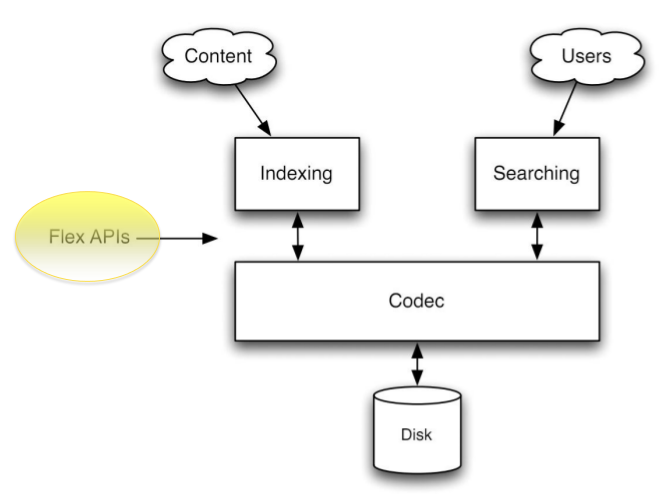
\includegraphics[scale=0.5]{pictures/architecture.png}
 \caption{Schemat architektury opartej o kodeki. Źródło: \cite{flexindex}.\label{fig:newarchitecture}}
\end{figure}

Operacje na indeksie (dodawanie, usuwanie lub modyfikowanie dokumentów, wyszukiwanie) są obecnie zaimplementowane w wyższych warstwach biblioteki (co ilustrują bloki \emph{Indexing} i \emph{Searching} na rys. \ref{fig:newarchitecture}). Kodek dostarcza formatu narzędzi do zapisu i odczytu zaindeksowanych dokumentów. Poprzez jego podmianę można zastosować np. niestandardowe algorytmy kompresji, nowe struktury danych do przechowywania słowników termów itp.

Wspomniane już oddzielenie logiki od formatu indeksu (konkretnych formatów plików przechowujących zaindeksowane dane) jest realizowane następująco. Moduły odpowiedzialne za indeksowanie i wyszukiwanie operują jedynie na reprezentacji indeksu: abstrakcyjnych klasach reprezentujących pola, termy bądź pojedyncze postingi. Nie odnoszą się w ogóle do sposobu zapisu i odczytu informacji: ,,nie wiedzą'' nic o algorytmach kompresji czy strukturach użytych do efektywnego przechowywania danych na dysku. Abstrakcyjna struktura indeksu jest przedstawiona na rys. \ref{fig:4dimAPI} i \ref{fig:indexApi} oraz omówiona w sekcji \ref{sec:4dimAPI}.

Kodek natomiast zawiera ,,ukonkretnione'' (nieabstrakcyjne) rozszerzenia tych klas. W związku z tym wszystkie wspólne operacje związane z indeksowaniem i wyszukiwaniem są zaimplementowane w abstrakcyjnych klasach z diagramu \ref{fig:indexApi}. Natomiast operacje związane z faktycznym zapisem i odczytem danych z dysku są realizowane w klasach kodeka. 

Kodek sam w sobie nie dodaje nowych możliwości bibliotece. Pozwala za to na efektywną (lub: efektywniejszą niż domyślna) realizację indeksowania i wyszukiwania, poprzez zastosowanie ,,niskopoziomowych'' mechanizmów optymalizacji. Struktura klas abstrakcyjnych przedstawiona na diagramie \ref{fig:indexApi} należy do części biblioteki odpowiedzialnej za indeksowanie -- niezależnej od kodeka. Klasy kodekowe odpowiedzialne są za dostarczenie mechanizmów pozwalających na wykonanie tych operacji przy wykorzystaniu konkretnego formatu kodowania danych. Dlatego właśnie mówimy, że kodek pośredniczy pomiędzy logiką indeksu a dyskowym formatem danych.

\section{Struktura kodeka}
\label{sec:codecStructure}

Kodek jest klasą o rozszerzającą abstrakcyjny \texttt{Codec}. Konkretna implementacja jest podłączana do reszty biblioteki przy użyciu mechanizmu Java SPI (\emph{Java Service Provider Interface}). Istnieje w związku z tym możliwość wykorzystania własnego kodeka lub wyboru jednego z dostarczonych.

Klasa \texttt{Codec} gromadzi (i dostarcza) tzw. formaty: klasy odpowiedzialne za zapis i odczyt poszczególnych części indeksu. Każdy kodek składa się z ośmiu części, które luźno odpowiadają plikom zapisywanym na dysku (tzn. przyjmuje się, że każda część kodeka zapisuje i odczytuje swój plik -- nie jest to jednak konieczność). Podczas projektowania własnego kodeka istnieje możliwość łączenia istniejących rozwiązań z własnymi implementacjami -- można skorzystać z domyślnych implementacji większości elementów i podmienić np. tylko część odpowiedzialną za kodowanie list postingowych.

Elementy, na które składa się kodek to:
\begin{enumerate}
 \item format list postingowych (\texttt{PostingsFormat}),
 \item format DocValues (\texttt{DocValuesFormat}),
 \item format pól przechowywanych (\emph{stored fields}, \texttt{StoredFieldsFormat}),
 \item format dla \emph{term vectors} (\texttt{TermVectorsFormat}) -- \emph{term vectors} to, nieformalnie rzecz ujmując, miniaturowe indeksy odwrócone tworzone dla każdego dokumentu z osobna. Dzięki nim można np. wylistować wszystkie termy występujące w danym dokumencie, wraz z ich częstościami oraz pozycjami występowania. Dodanie tej funkcjonalności do głównego indeksu jest opcjonalne,
 \item format informacji o polach i związanych z tym statystyk (\texttt{FieldInfosFormat}),
 \item format zapisu ogólnych informacji dotyczących segmentów (\texttt{SegmentInfoFormat}),
 \item format zapisu \emph{norm} (\texttt{NormsFormat}) -- związanych z poszczególnymi polami liczb wskazujących, czy dane pole powinno być traktowane jako mniej lub bardziej istotne niż pozostałe (są to zagregowane wskaźniki \emph{boost} zapisywanie podczas indeksowania, wspomniane w sekcji \ref{sec:boosting}),
 \item format do zapisu informacji o tym, które dokumenty powinny zostać usunięte podczas najbliższej optymalizacji indeksu (\texttt{LiveDocsFormat}).
\end{enumerate}

\section{Czterowymiarowa struktura indeksu}
\label{sec:4dimAPI}

Zmiany, poza rozdzieleniem formatu zapisu indeksu do plików od architektury, dotyczyły także interfejsu programisty. Dostęp do poszczególnych elementów indeksu, czyli pól, termów, numerów dokumentów, pozycji wystąpień termu w dokumencie, itp. odbywa się przy pomocy tzw. \emph{czterowymiarowego API}, które obrazowo przedstawione jest na rys. \ref{fig:4dimAPI}.

\begin{figure}[here]
 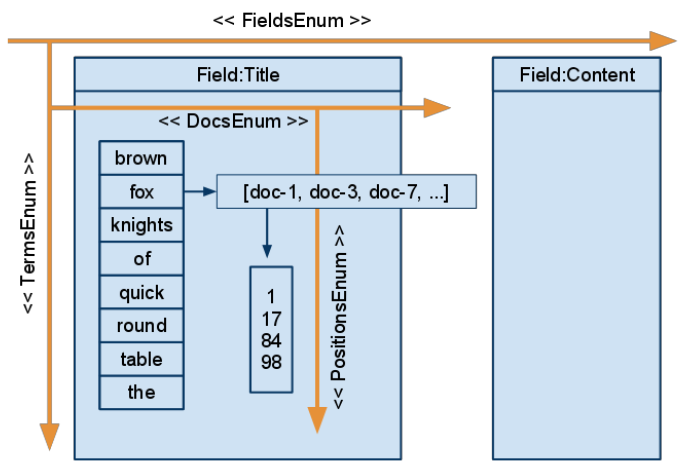
\includegraphics[scale=0.5]{pictures/api.png}
 \caption{Schemat interfejsu programisty pozwalającego na dostęp do poszczególnych elementów indeksu. Źródło: \cite{flexindex}.\label{fig:4dimAPI}}
\end{figure}

Najbardziej nadrzędnym elementem dostępu do indeksu jest pole (\texttt{Field}). W uproszczeniu, dla każdego indeksu (bądź jego abstrakcji) możemy pobrać listę jego pól (przedstawione tutaj jako \texttt{FieldsEnum}, implementowane jako \texttt{Fields} -- o czym będzie mowa w dalszej części tego rozdziału). Pole, poza tytułem, posiada listę termów, do której mamy dostęp poprzez iterator \texttt{TermsEnum}. Dla każdego termu możemy pobrać listę dokumentów, w których on wystąpił (\texttt{DocsEnum}), a dla każdego z dokumentów -- listę pozycji wystąpień (\texttt{PositionsEnum} -- jak zostanie to omówione później, w faktycznej implementacji iteratory \texttt{DocsEnum} i \texttt{PositionsEnum} są zaimplementowane jako jedna klasa).

Schemat \ref{fig:4dimAPI} nie oddaje faktycznej architektury dostępu do elementów indeksu -- jest jedynie jej nakreśleniem. Rysunek poniżej (\ref{fig:indexApi}) ilustruje, w jaki sposób koncepcja czterowymiarowego API została przełożona na abstrakcyjne klasy Lucene Core, biorące udział w procesie indeksowania i wyszukiwania. Diagram ten ilustruje także powiązania pomiędzy klasami -- stanowi definicję serwisu (posługując się definicją Java SPI, jest to \emph{Service Interface}). Zatem programista chcący zaimplementować własny kodek musi stworzyć swoją hierarchię klas zgodnie z tą strukturą i narzuconymi funkcjami jej poszczególnych elementów (np. poprzez ich rozszerzenie).

\begin{figure}[here]
 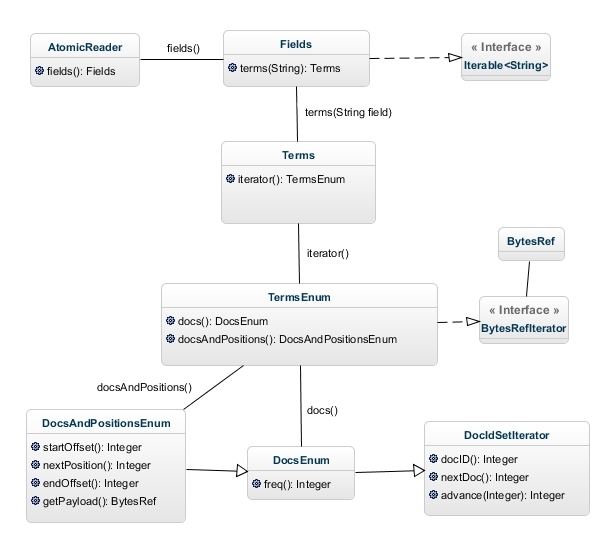
\includegraphics[scale=0.64]{pictures/LuceneAccessAPI_1.jpg}
 \caption{Struktura klas służących do pobierania poszczególnych elementów indeksu. Źródło: opracowanie własne.\label{fig:indexApi}}
\end{figure}

Jak zostało to wcześniej wspomniane, pola są najwyższą warstwą w hierarchii dostępu do danych indeksu. Są one od siebie niezależne do tego stopnia, że istnieje możliwość takiego skonfigurowania indeksu, aby każde pole było kodowane przy pomocy innego kodeka. W konsekwencji możemy więc myśleć o indeksie zawierającym wiele pól jako o kilku równoległych indeksach. To także ma wpływ na sposób traktowania termów: ten sam term, ale znajdujący się w dwóch różnych polach jest traktowany jako dwa osobne termy. Stąd wynika powtarzana już wcześniej uwaga o tym, że każdy term jest identyfikowany przez swój token oraz nazwę pola, do którego należy.

Zajmijmy się teraz omówieniem poszczególnych klas diagramu \ref{fig:indexApi} i ich ról w procesie odczytu i zapisu danych do indeksu. \texttt{AtomicReader} jest abstrakcyjnym rozszerzeniem \texttt{IndexReadera} pozwalającym na dostęp do informacji przechowywanych w indeksie odwróconym -- w szczególności do jego pól (\texttt{IndexReader} sam w sobie nie posiada takiej funkcjonalności -- podobnie jak niektóre jego klasy potomne. Zagadnienie to jest szerzej omówione w sekcji \ref{sec:indexReader}). 

\texttt{AtomicReader} potrafi zwrócić obiekt \texttt{Fields}, implementujący interfejs iteratora napisów (\texttt{Iterable<String>}, pochodzący ze standardowej biblioteki Javy). Oznacza to, że \texttt{Fields.iterator()} przechodzi po wszystkich nazwach pól znajdujących się w indeksie. Z obiektu \texttt{Fields} można pobrać obiekt \texttt{Terms}, który poza iteratorem termów (\texttt{TermsEnum}) zawiera także statystyki dotyczące wszystkich termów pola (liczba dokumentów, w których ten term występuje, łączna liczba wystąpień termu w polu, itp.).

Od wersji 4.0 Lucene term (a konkretniej -- jego token) jest reprezentowany jako ciąg bajtów (a nie, jak wcześniej, jako napis w kodowaniu UTF-16). Pozwala to na uniknięcie problemów związanych z kodowaniem znaków, szczególnie w językach wschodnioazjatyckich -- odpowiedzialność za kodowanie i odkodowywanie znaków z ciągu bajtów jest przerzucona na kodek -- wyższe warstwy biblioteki ,,widzą'' tylko opakowanie ciągu bajtów. Klasą wykorzystaną do reprezentacji takiego ciągu jest \texttt{BytesRef} (który tak naprawdę przechowuje informacje o początku danego podciągu oraz jego długości w większej tablicy typu \texttt{byte[]}).

Zauważmy, że \texttt{TermsEnum} implementuje interfejs \texttt{BytesRefIterator}. Oznacza to tyle, że jest on w stanie wylistować wszystkie przechowywane termy. Tę samą funkcjonalność można byłoby uzyskać wykorzystując standardowy iterator dla Javy (\texttt{TermsEnum} mogłoby implementować \texttt{Iterable<BytesRef>}). Wygląda na to, że wprowadzanie dodatkowej klasy, \texttt{BytesRefIterator}, jest niepotrzebne i powoduje tylko spadek czytelności kodu.

W zależności od tego, czy podczas indeksowania dla każdego wystąpienia termu zostały zapisane dodatkowe informacje (pozycje wystąpień, \emph{payloads}), do wylistowania dokumentów, w których wystąpił dany term można użyć jednej z dwóch abstrakcji: \texttt{DocsEnum} lub rozszerzającego \texttt{DocsAndPositionsEnum}. Obydwie klasy są dostępne z poziomu obiektu \texttt{TermsEnum} -- dla termu wskazywanego obecnie przez iterator istnieje możliwość pobrania tak opakowanej listy dokumentów.

Zauważmy, że do wylistowania wszystkich dokumentów z \texttt{DocsEnum} wykorzystany jest kolejny interfejs iteratora: \texttt{DocIdSetIterator}. W tym wypadku wprowadzenie dodatkowej klasy dla tej samej funkcjonalności wydaje się jednak uzasadnione: \texttt{DocIdSetIterator}, poza standardowymi funkcjami iteratora, pozwala na przejście do wskazanego elementu listy (abstrakcyjne metody \texttt{advance(int target)} oraz \texttt{slowAdvance(int target)}: dokumentacja sugeruje, aby implementacja pierwszej z nich wykorzystywała skip listy).

\section{Dostęp do plików indeksu: \texttt{IndexReader} i jego implementacje}
\label{sec:indexReader}

Pliki indeksu w najczęstszym przypadku przechowywane są w jednym katalogu dyskowym. Nic jednak nie stoi na przeszkodzie, aby indeks był rozproszony pomiędzy wiele folderów lub maszyn lub żeby był przechowywany w pamięci RAM (takie rozwiązanie zostało już zaprezentowane w rozdziale pierszym. Stosuje się je często w celach testowych).

W przykładzie z pierwszego rozdziału przedstawiono prosty odczyt indeksu przy pomocy klas \texttt{IndexReader} i \texttt{DirectoryReader}. W tej sekcji omówione zostaną także inne sposoby dostępu do indeksu w Lucene. Schemat klas implementujących tę funkcjonalność przedstawia rys. \ref{fig:indexReader}. 

\begin{figure}[p]
 \centering
 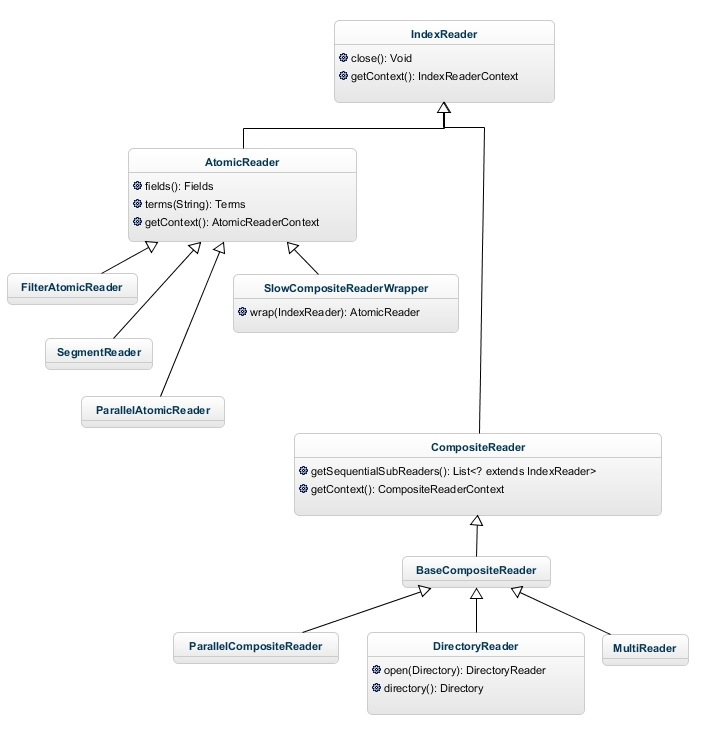
\includegraphics[scale=0.64]{pictures/Readers_1.jpg}
 \caption{Struktura klas dostępu do indeksu: \texttt{IndexReader} oraz klasy potomne. Źródło: opracowanie własne. \label{fig:indexReader}}
\end{figure}

Abstrakcyjny \texttt{IndexReader}, stojący na szczycie tej hierarchii, dostarcza tylko najbardziej podstawowych funkcji, wspólnych wszystkim klasom odczytującym (takich jak zamykanie indeksu -- metoda \texttt{close()}, obliczanie prostych statystyk: liczby dokumentów w indeksie, informacji o tym, czy dany indeks posiada dokumenty usunięte, itp.). 

\texttt{IndexReader} nie ma dostępu do zawartości indeksu odwróconego -- poprzez jego interfejs można uzyskać jedynie wartości pól przechowywanych (\emph{stored fields}). Wszystkie inne zaindeksowane informacje muszą być pobrane przy pomocy jego rozszerzeń. Taka decyzja architektoniczna podyktowana jest chęcią uproszczenia procesu wyszukiwania z punktu widzenia programisty: użytkownik Lucene (najczęściej program wykorzystujący Lucene do wyszukiwania tekstowego) nie musi tak naprawdę nic wiedzieć o indeksie odwróconym, zaindeksowanych termach czy listach postingowych. Wystarczy, że poda bibliotece odpowiednio skonstruowane zapytanie i odbierze wyniki w postaci listy referencji do pasujących dokumentów (wartości pól przechowywanych mogą być mu przydatne do zaprezentowania wyników). Zatem projektanci Lucene zdecydowali, że najogólniejsza klasa dostępu do indeksu będzie posiadała odpowiednio ograniczone funkcjonalności.

Z \texttt{IndexReadera} wywiedzione są dwie abstrakcyjne klasy: \texttt{AtomicReader} oraz \texttt{CompositeReader}. \texttt{AtomicReader} umożliwia dostęp do indeksu na poziomie segmentu. To właśnie on pozwala na pobranie informacji o indeksie odwróconym. Dlatego, m.in., jego implementacje (najczęściej \texttt{SegmentReader}) są niezbędne podczas łączenia segmentów i innych wewnętrznych operacji.

Ponieważ w większości przypadków indeks składa się z kilkunastu -- kilkudziesięciu segmentów, użytkownicy Lucene rzadko odwołują się bezpośrednio do instancji typu \texttt{AtomicReader}. Dużo bardziej przydatne okazuje się wykorzystanie \texttt{CompositeReaderów}, z których najbardziej popularnym jest \texttt{DirectoryReader}. Klasy wywiedzione z \texttt{CompositeReadera} nie dostarczają żadnych nowych funkcjonalności w stosunku do \texttt{IndexReadera} -- tak samo, nie pozwalają na dostęp do indeksu odwróconego. Implementują jednak dostęp do ,,łączonych indeksów'', dyskowych lub rozproszonych: agregują inne rozszerzenia klasy \texttt{IndexReader} i np. pobieranie informacji z list postingowych przekazują do odpowiednich \texttt{AtomicReaderów}. Są przykładem implementacji wzorca projektowego o nazwie kompozyt.

\texttt{CompositeReaders} pozwalają na bezpośredni dostęp do swoich elementów: można je wylistować przy pomocy metody \texttt{CompositeReader.getSequentialSubReaders()}. Zatem programista chcący uzyskać np. listę termów zaindeksowanych w indeksie dyskowym ma możliwość odczytania list z poszczególnych ,,readerów atomowych''.

Innym sposobem uzyskania funkcjonalności \texttt{AtomicReadera} dla ,,readera złożonego'' jest skorzystanie z klasy \texttt{SlowCompositeReaderWrapper}, która poprzez metodę \texttt{wrap()} przyjmuje instancję \texttt{CompositeReadera} i w wyniku zwraca obiekt ,,udający'' \texttt{AtomicReader}. Wewnątrz sekwencyjnie ,,przechodzi'' po wszystkich zagregowanych \texttt{AtomicReaderach} i w locie łączy pobrane z nich dane. Dokumentacja Lucene odradza jednak korzystanie z tego rozwiązania, ze względu na potencjalnie długi czas wykonywania różnych operacji.

\subsection{\texttt{IndexReaderContext}}

W działającym programie wykorzystującym Lucene instancje typu \texttt{IndexReader} tworzą strukturę drzewiastą, w której węzłami są implementacje klasy \texttt{CompositeReader} a liśćmi -- implementacje \texttt {AtomicReadera}. Każdy element tej struktury posiada informacje o ,,swoim'' fragmencie indeksu (swoim segmencie, katalogu z plikami indeksu, itp.). W związku z tym, że np. dodawane dokumenty są indeksowane od zera w obrębie każdego segmentu, mogą wystąpić problemy ze spójnością numeracji wewnątrz \texttt{CompositeReaderów}. Projektanci biblioteki musieli wobec tego zdecydować, której klasie przydzielona zostanie odpowiedzialność za zarządzanie całą strukturą. Między innymi, rozwiązania wymagały następujące problemy: 
\begin{itemize}  
 \item która klasa ma pamiętać kolejność \texttt{AtomicReaderów} wewnątrz kompozytu?
 \item gdzie powinny być przechowywane podstawy przenumerowania dokumentów z danego segmentu?
\end{itemize}
Trzymanie takich informacji wewnątrz \texttt{CompositeReadera} byłoby naruszeniem zasad projektowania obiektowego (w szczególności, zasady SRP -- \emph{Single Responsibility Principle}).

Eleganckim rozwiązaniem w tym wypadku okazało się wprowadzenie dodatkowej hierarchii klas -- tzw. kontekstów. Ich zadaniem jest przechowywanie informacji o strukturze i kolejności klas odczytujących indeks. Każda instancja typu \texttt{IndexReader} posiada obiekt \texttt{IndexReaderContext} (lub wywiedziony). Hierarchia kontekstów oraz możliwe na niej operacje są przedstawione na rys. \ref{fig:indexReaderContexts}. 

\begin{figure}[here]
 \centering
 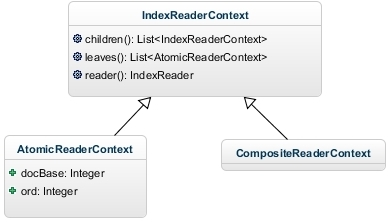
\includegraphics[scale=0.7]{pictures/ReaderContexts.jpg}
 \caption{Struktura kontekstów \texttt{IndexReader}. Źródło: opracowanie własne. \label{fig:indexReaderContexts}}
\end{figure}

Każdy \texttt{IndexReaderContext} potrafi wylistować konteksty readerów potomnych, konteksty liści drzewa readerów oraz wskazać konkretną instancję typu \texttt{IndexReader}, do której jest przypisany. Dodatkowo, konteksty instancji \texttt{AtomicReader} pamiętają wartość \texttt{docBase} -- bazę przenumerowania dokumentów oraz swój numer w wewnętrznej tablicy nadrzędnego \texttt{CompositeReadera} (wartość \texttt{ord}). Dzięki temu wiadomo, w jakiej kolejności powinny być przeglądane poszczególne instancje typu \texttt{IndexReader}.

\section{Implementacja własnego kodeka}

Format list postingowych jest miejscem, które najprawdopodobniej zmieniłby programista chcący zaimplementować np. nowy algorytm kompresji postingów czy reprezentacji termów. Dlatego zajmiemy się teraz opisem architektury tej części kodeka. 

Jak zostało wspomniane w sekcji \ref{sec:codecStructure}, za format list postingowych odpowiada klasa \texttt{PostingsFormat}. Jej głównym zadaniem jest dostarczenie i zarządzanie cyklem życia dwóch obiektów: \texttt{FieldsProducer} i \texttt{FieldsConsumer}, które są odpowiedzialne za, odpowiednio, odczyt i zapis danych z plików indeksu. Architekturę formatu list postingowych przedstawia rys. \ref{fig:postingFormat}.

\begin{figure}[p]
 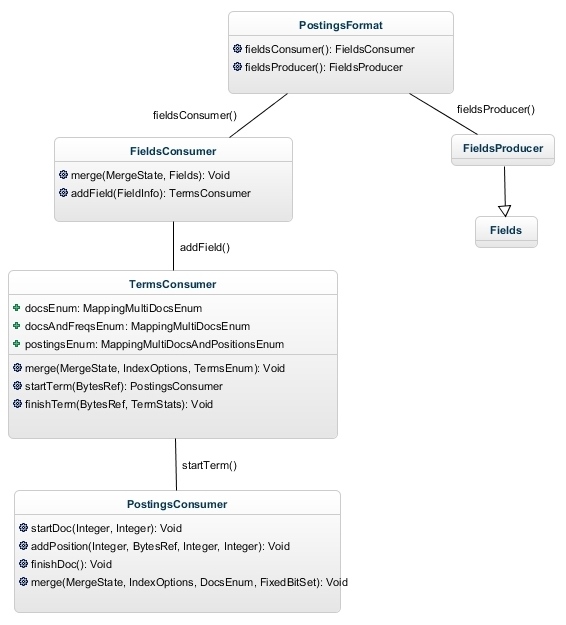
\includegraphics[scale=0.65]{pictures/PostingsFormat_1.jpg}
 \caption{Schemat klas służących do zapisu formatu list postingowych. Źródło: opracowanie własne.\label{fig:postingFormat}}
\end{figure}

Klasa \texttt{FieldsProducer} jest odpowiedzialna za odczyt danych z segmentu -- stąd powiązanie z przedstawioną już wcześniej klasą \texttt{Fields}. \texttt{FieldsConsumer} jest z kolei odpowiedzialny za zapis nowego segmentu (powstałego w wyniku zrzutu danych na dysk lub w wyniku łączenia segmentów niższego poziomu). Określenia \emph{producer} i \emph{consumer} mogą wydawać się tutaj mało intuicyjne. Zrozumienie ich ról może ułatwić następujące zdanie: ,,\texttt{FieldsConsumer} \emph{pobiera} (konsumuje) właśnie definiowane pole i zapisuje je w indeksie, podczas gdy \texttt{FieldsProducer} odczytuje pole z indeksu (\emph{produkuje} je z plików indeksu)''.

Dodawanie nowych pól do instancji \texttt{FieldsConsumera} odbywa się za pomocą metody \texttt{addField()} przyjmującej jako parametr obiekt typu \texttt{FieldInfo}, przechowujący informacje o konfiguracji pola (takie jak jego wewnętrzny numer, nazwę, opcje indeksowania, atrybuty, itp.). Metoda ta zwraca obiekt \texttt{TermsConsumer}, pozwalający na dodawanie termów do pola. \texttt{TermsConsumer} posiada trzy atrybuty typu \texttt{DocsEnum} (a konkretniej: typów rozszerzających \texttt{DocsEnum}). Są one wykorzystywane podczas łączenia segmentów -- w zależności od opcji indeksowania, wybierany jest jeden a nich i pełni on rolę iteratora dokumentów.

Wywołanie \texttt{TermsConsumer.startTerm()} zwraca obiekt \texttt{PostingsConsumer}, który, operując już na numerach dokumentów i pozycjach występowania danego termu, zapisuje listy postingowe.

Oczywiście, wszystkie klasy diagramu \ref{fig:postingFormat} są abstrakcyjne. Wspomniane wyżej metody często są jedynie zadeklarowane w odpowiednich klasach. Operacje takie jak dodawanie pola, termu lub dokumentu są ściśle związane z formatem kodowania indeksu i w związku z tym muszą być oprogramowane w kodeku. Co za tym idzie, każdy kodek będzie posiadał własne rozszerzenia klas typu \texttt{Producer} i \texttt{Consumer} oraz wszystkich iteratorów. 

Klasy \texttt{FieldsConsumer}, \texttt{TermsConsumer}, \texttt{PostingsConsumer} posiadają jedynie implementacje metod \texttt{merge()}: według projektantów Lucene łączenie poszczególnych elementów indeksu powinno być niezależne od faktycznego formatu zapisu. Nic jednak nie stoi na przeszkodzie, aby kodek nadpisywał także tę funkcjonalność.

\subsection{Zapis i odczyt indeksu w domyślnym kodeku}

Należy pamiętać, że powiązania pomiędzy klasami i funkcjonalności zaprezentowane na \ref{fig:indexApi} i \ref{fig:postingFormat} są jedynie definicjami usługi (posługując się znów terminologią związaną z Java SPI). Faktyczne realizacje klas okazują się być bardziej skomplikowane. Rysunek \ref{fig:postingFormatRead} przedstawia strukturę klas do odczytu danych z indeksu wykorzystywaną w obecnie domyślnym kodeku. Przyjrzyjmy się jej bliżej.

\texttt{BlockTreeTermsReader} jest realizacją klasy \texttt{FieldsProducer} -- jest więc odpowiedzialny za wyliczanie termów należących do danego pola. Jego nazwa wywodzi się z tego, że słownik termów w obecnej wersji Lucene jest trzymany w postaci zbioru bloków, co powoduje przyspieszenie odczytu i zapisu danych (operujemy na blokach danych, a nie na pojedynczych wartościach). 

\texttt{BlockTreeTermsReader}, jako implementacja \texttt{FieldsProducera}, będzie przechowywał termy odczytane dla danego pola w obiektach typu \texttt{Terms} i \texttt{TermsEnum}. Dla domyślnego kodeka, ukonkretnieniem \texttt{Terms} jest \texttt{FieldReader}, a ukonkretnieniem \texttt{TermsEnum} -- \texttt{SegmentTermsEnum} (por. relacje dziedziczenia po prawej stronie diagramu \ref{fig:postingFormatRead}). \texttt{FieldsReader} jest klasą wewnętrzną \texttt{BlockTreeTermsReadera}, a \texttt{SegmentTermsEnum} -- klasą wewnętrzną \texttt{FieldsReadera}. 

Ponadto, \texttt{BlockTreeTermsReader} agreguje instancję typu \texttt{PostingsReaderBase}. W przypadku domyślnego kodeka jej realizacją jest \texttt{Lucene41PostingsReader}. \texttt{PostingsReaderBase} pełni rolę pośrednika pomiędzy klasą \texttt{SegmentTermsEnum}, odpowiedzialną za dostarczanie kolejnych odczytanych termów a klasą \texttt{Lucene41PostingsReader}, odpowiedzialną za odczyt samych list postingowych dla konkretnego termu. 

Zauważmy, że samo \texttt{PostingsReaderBase} (a co za tym idzie, także -- \texttt{Lucene41PostingsReader}) nie rozszerzają \texttt{TermsEnum}. Nie dziedziczą więc ,,domyślnej'' możliwości tworzenia iteratorów numerów dokumentów (jak pamiętamy z diagramu \ref{fig:indexApi} i sekcji \ref{sec:4dimAPI}, \texttt{TermsEnum} tworzy takowe iteratory -- są nimi \texttt{DocsEnum} lub \texttt{DocsAndPositionsEnum}). Jednak nieprzypadkowo \texttt{PostingsReaderBase} posiada metody \texttt{docs()} oraz \texttt{docsAndPositions()} -- o takiej samej sygnaturze, jak składowe klasy \texttt{TermsEnum}. \texttt{SegmentTermsEnum} \emph{deleguje} bowiem pobranie list dokumentów dla danego termu do instancji klasy \texttt{PostingsReaderBase}.

Takie rozwiązanie pozwala na oddzielenie odczytu pól oraz słownika termów (za co odpowiada sam \texttt{BlockTreeTermsReader}) od odczytu list postingowych. Ponieważ \texttt{PostingsReaderBase} jest \emph{wstrzykiwany} poprzez konstruktor do \texttt{BlockTreeTermsReader}, \texttt{BlockTreeTermsReader} nie będzie tworzył i zarządzał cyklem życia klasy odczytującej postingi. A co za tym idzie -- tę ostatnią można łatwo podmienić.

Ponadto, dzięki takiemu rozwiązaniu w kodeku może istnieć kilka klas odczytujących postingi. Wszystkie one rozszerzałyby \texttt{PostingsReaderBase}, byłyby więc uniezależnione od ogólnej architektury przedstawionej na \ref{fig:indexApi}. Oczywiście, tylko jedna z nich byłaby w danym uruchomieniu używana.

\begin{figure}[p]
 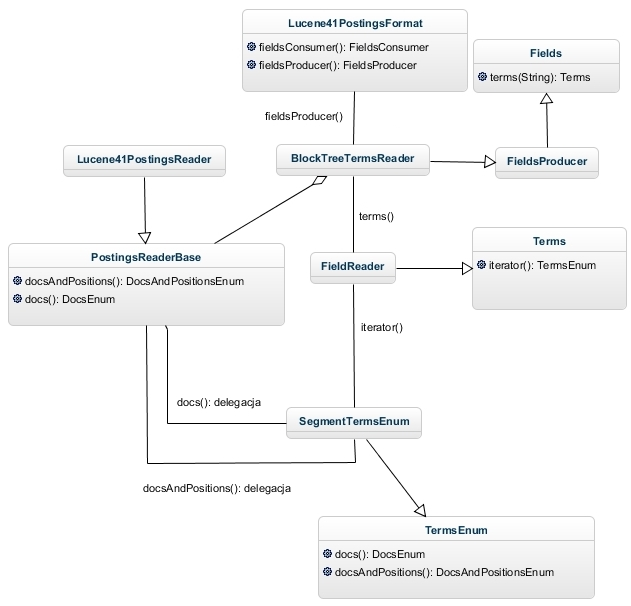
\includegraphics[scale=0.67]{pictures/Lucene41PostingsFormatRead_2.jpg}
 \caption{Odczyt list postingowych i innych informacji z indeksu odwróconego: schemat klas wykorzystywanych przez domyślny kodek. Źródło: opracowanie własne. \label{fig:postingFormatRead}}
\end{figure}

W przypadku zapisu mamy do czynienia z podobną sytuacją: dzięki wstrzykiwaniu instancji typu \texttt{PostingsWriterBase} do \texttt{BlockTreeTermsWriter}, zapis list postingowych jest niezależny od zapisu pól i słownika termów.

Jak przedstawione jest to na diagramie \ref{fig:postingFormatWrite}, \texttt{BlockTreeTermsWriter} agreguje instancję typu \texttt{PostingsWriterBase}, która jest odpowiedzialna za zapis list postingowych do plików. W przypadku domyślnego kodeka jest nią \texttt{Lucene41PostingsWriter}. \texttt{BlockTreeTermsWriter}, jako ukonkretnienie \texttt{FieldsConsumera}, przy okazji dodawania nowego pola tworzy obiekt typu \texttt{TermsConsumer}, dzięki któremu możliwy będzie zapis termów do właśnie utworzonego pola. Ukonkretnieniem abstrakcyjnego \texttt{TermsConsumera} jest tutaj \texttt{TermsWriter} -- wewnętrzna klasa \texttt{BlockTreeTermsWritera}.

Jak zostało to już wspomniane w \ref{sec:4dimAPI}, zapis termu rozpoczyna się poprzez wywołanie metody \texttt{startTerm()}, z której zwrócona zostaje instancja typu \texttt{PostingsConsumer}. \texttt{TermsWriter} deleguje wywołanie tej metody do przechowywanej przez \texttt{BlockTreeTermsWriter} instancji \texttt{PostingsWriterBase}, a następnie ją zwraca. Dzięki temu schemat zapisu jest zachowany, a jednocześnie możliwa jest podmiana klasy odpowiedzialnej za zapis postingów.

Widać zatem, że skomplikowanie architektury zapisu danych do indeksu ma ten sam cel, co opisane wcześniej skomplikowanie architektury odczytu: uniezależnia klasę zapisującą pola i słownik termów od klasy zapisującej listy postingowe. Dzięki wprowadzeniu dodatkowego pośrednika -- \texttt{PostingsWriterBase} -- dużo łatwiej byłoby podmienić obecnie używany \texttt{Lucene41PostingsWriter}, gdyby zaszła taka potrzeba.

\begin{figure}[p]
 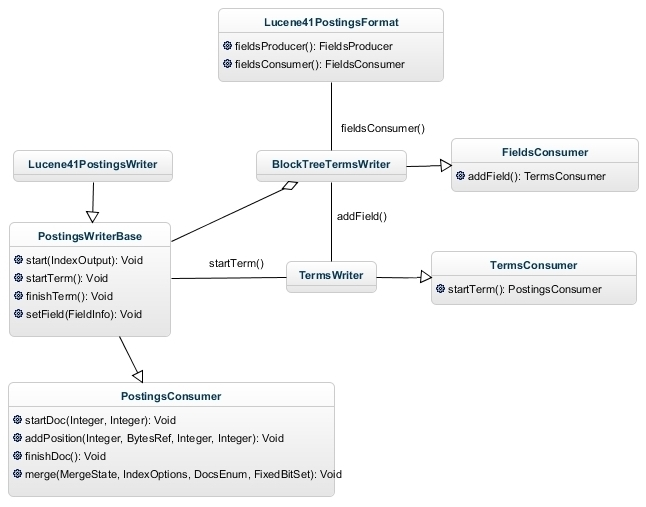
\includegraphics[scale=0.65]{pictures/Lucene41PostingsFormatWrite_1.jpg}
 \caption{Zapis list postingowych i innych informacji do indeksu odwróconego: schemat klas wykorzystywanych przez domyślny kodek. Źródło: opracowanie własne. \label{fig:postingFormatWrite}}
\end{figure}

\section{Format list postingowych}

W tym podrozdziale opisany zostanie obecnie stosowany format list postingowych (dla domyślnego kodeka używanego w Lucene od wersji 4.1) Schematyczne przedstawienie tego formatu znajduje się na rys. \ref{fig:postingCodingFormat}.

\begin{figure}[here]
 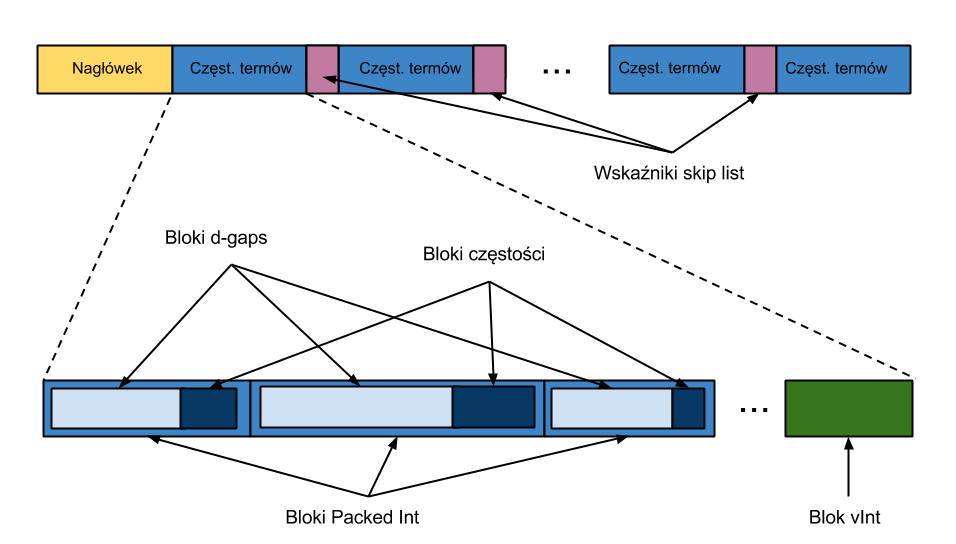
\includegraphics[scale=0.37]{pictures/PostingCodingFormat.png}
 \caption{Schematyczne przedstawienie sposobu zapisu list postingowych. Źródło: opracowanie własne. \label{fig:postingCodingFormat}}
\end{figure}

Elementami list postingowych są różnice pomiędzy numerami dokumentów (zwane dalej \emph{d-gaps} lub \emph{DocDelta}). Na liście postingowej może być dodatkowo przechowywana informacja o liczbe wystąpień danego termu w dokumencie.

Listy postingowe kodowane są blokami dwóch rodzajów. Wszystkie bloki (być może poza ostatnim) są blokami tzw. upakowanymi (\emph{Packed Blocks}). Liczba postingów w takim bloku jest stała i wynosi 128. Jeśli liczba postingów w liście nie jest podzielna przez 128, pozostałe postingi (te, które nie zmieściły się w ostatnim bloku upakowanym) są zapisywane w postaci dodatkowego bloku i są kodowane przy pomocy starego formatu liczb całkowitych o zmiennej długości \texttt{vInt}.

Lista postingowa jest skip listą, w której blok jest najmniejszą jednostką, o którą można ,,przeskoczyć''. Wskaźniki skip list zapisywane są na początku każdego bloku (z wyjątkiem pierwszego).

\subsection{Kodowanie bloków upakowanych}
\label{sec:packedBlockEncoding}

Każdy blok upakowany (\emph{PackedBlock}) składa się z dwóch części: 
\begin{enumerate}
 \item upakowanych numerów dokumentów (\emph{PackedDocDeltaBlock}, bloki upakowanych \emph{d-gaps}),
 \item (opcjonalnie) części kodującej częstości wystąpienia danego termu w dokumencie (\emph{PackedFreqBlock}, bloki częstości).
\end{enumerate}

Algorytm kodowania numerów dokumentów w bloku upakowanym jest bardzo prosty: najpierw obliczane są różnice pomiędzy kolejnymi numerami dokumentów (tzw. \emph{d-gaps}), a następnie kolejne grupy po 128 postingów są osobno kodowane jako blok upakowany. Dla każdej grupy \emph{d-gaps}, która ma zostać zakodowana jako blok, wybierana jest minimalna liczba bitów, przy pomocy której wszystkie z nich będą mogły zostać przedstawione. Informacja o tej liczbie zapisywana jest w pierwszym bajcie bloku. Następnie zapisywany jest ciąg zakodowanych \emph{d-gaps}.

Dodatkowo, jeśli wszystkie \emph{d-gaps} są takie same (np. jeśli dany term występuje we wszystkich dokumentach i w związku z tym wszystkie \emph{d-gaps} mają wartość 1), w pierwszym bajcie bloku zapisywana jest wartość 0, a następnie -- powtarzająca się liczba jako pojedynczy \texttt{vInt}.

Wedle podobnego schematu kodowana jest część zawierająca częstości wystąpień termu w dokumencie -- z pominięciem obliczania \emph{d-gaps}, które tutaj nie są potrzebne.

\subsection{Kodowanie \texttt{vInt}}
\label{sec:vIntEncoding}

W tym formacie kodowania informacje o numerze dokumentu oraz o częstości występowania termu są zakodowane naprzemiennie (tzn. jeśli częstość występowania termu w danym dokumencie jest większa niż 1, kodowana jest jako kolejna liczba na liście). 

Elementy tego bloku nazywane się \emph{DocDelta} i kodowane są jako liczby \texttt{vInt}. Kodowaniem tym rządzą następujące reguły:
\begin{itemize}
 \item jeśli częstości występowania termu są zaindeksowane, wartość \emph{DocDelta} zawiera informacje zarówno o \emph{d-gap} jak i o częstości,
 \item $\emph{d-gap} = \emph{DocDelta} / 2$ (dzielenie bez reszty)
 \item jeśli $\emph{DocDelta}~\%~2 = 1$, to częstość termu wynosi 1,
 \item jeśli $\emph{DocDelta}~\%~2 = 0$, to częstość występowania termu zakodowana jest jako kolejna liczba (\texttt{vInt}) na liście.
\end{itemize}

Kodowanie liczb \texttt{vInt} odbywa się według podobnego algorytmu, jak opisany w \cite{irbook} w rozdziale 5.3.1 ,,Variable byte encodes''. Pierwszy bit każdego bajtu jest bitem kontynuacji: jeśli jego wartością jest 0, dany bajt jest ostatnim w liczbie. Pozostałe 7 bitów jest faktycznym kodowaniem danej pozycji w liczbie całkowitej: wartości kolejnych bajtów przekładają się na pozycje w systemie o podstawie 128.
\chapter{Algorytm łączenia segmentów}

Niezależnie od formatu zapisu plików indeksu, łączenie segmentów odbywa się według tego samego algorytmu. Za proces ten odpowiedzialna jest metoda \texttt{merge()} klasy \texttt{SegmentMerger} (klasa ta nie jest widoczna poza swoim pakietem -- nie można jej nadpisać ani rozszerzyć w implementacji swojego kodeka). Oto kolejność łączenia poszczególnych elementów segmentu:
\begin{enumerate}
 \item łączenie \texttt{FieldInfos} -- metadanych związanych z poszczególnymi polami,
 \item łączenie \texttt{StoredFields}, pól przechowywanych,
 \item \label{item:postingMerge} łączenie \texttt{Terms}: łączenie list postingowych dla poszczególnych termów w ramach jednego pola,
 \item łączenie \texttt{DocValues} (o ile zostały zaindeksowane),
 \item łączenie norm (o ile zostały zaindeksowane),
 \item łączenie \texttt{TermVectors} (o ile zostały zaindeksowane).
\end{enumerate}

%\section{Algorytm łączenia termów}
%
Łączenie termów i następujące w związku z nim łączenie list postingowych jest najważniejszym elementem całego procesu. Przyjrzymy mu się dokładniej.

Owo łączenie przebiega rekurencyjnie, po strukturze indeksu przedstawionej na rys. \ref{fig:indexApi}. Oznacza to, że najpierw łączone są definicje pól w obrębie zbioru łączonych segmentów. Jeśli dane pole występuje w więcej niż jednym segmencie, to w jego obrębie łączone są wszystkie termy. Analogicznie, jeśli w dwóch segmentach występuje ten sam term we właśnie połączonym polu, łączone są listy postingowe dla tego termu.

\section{Łączenie pól}

Łączenie pól odbywa się w metodzie \texttt{merge()} klasy \texttt{FieldsConsumer}. Tam bowiem przekazywane jest sterowanie z \texttt{SegmentMerger.merge()} na etapie łączenia pól, termów i list postingowych (krok \ref{item:postingMerge} z poprzednej sekcji). 

Samo połączenie pól pochodzących z różnych segmentów polega na utworzeniu instancji typu \texttt{MultiFields}, co zilustrowane jest na rys. \ref{fig:fieldMerge}. Dla każdego z łączonych segmentów pobierana jest instancja typu \texttt{AtomicReader} (a dokładniej: \texttt{SegmentReader}, por. \ref{sec:indexReader}). Na jego podstawie utworzona zostaje instancja klasy \texttt{ReaderSlice}, przechowująca następujące informacje:
\begin{enumerate}
 \item \texttt{docBase}: pierwszy numer, jaki zostanie nadany dokumentowi pochodzącego z obecnego \texttt{AtomicReadera} i zapisanego w wynikowym segmencie. W obrębie jednego segmentu numery dokumentów (\emph{docId}) są unikalne i zaczynają się od 0. W związku z tym, podczas łączenia dokumenty z co najmniej jednego segmentu muszą zostać przenumerowane. Do tego właśnie służy \texttt{docBase}: zostanie ona dodana do wszystkich \emph{docId} danego segmentu. Wartość \texttt{docBase} dla pierwszego z łączonych segmentów wynosi 0, dla każdego kolejnego jest równa łącznej liczbie ,,żywych'' (nieusuniętych) dokumentów z poprzednich segmentów;
 \item \texttt{maxDoc}: liczba dokumentów zaindeksowanych w danym segmencie;
 \item \texttt{readerIndex}: numer porządkowy segmentu.
\end{enumerate}

Z każdego \texttt{AtomicReadera} pobrana jest także instancja \texttt{Fields}. Tablice z odpowiadającymi sobie instancjami \texttt{ReaderSlice} oraz \texttt{Fields} służą do zainicjalizowania klasy \texttt{MultiFields}, służącej jako agregat pól -- będzie ona wykorzystana w dalszej części procesu.

\begin{figure}[here]
 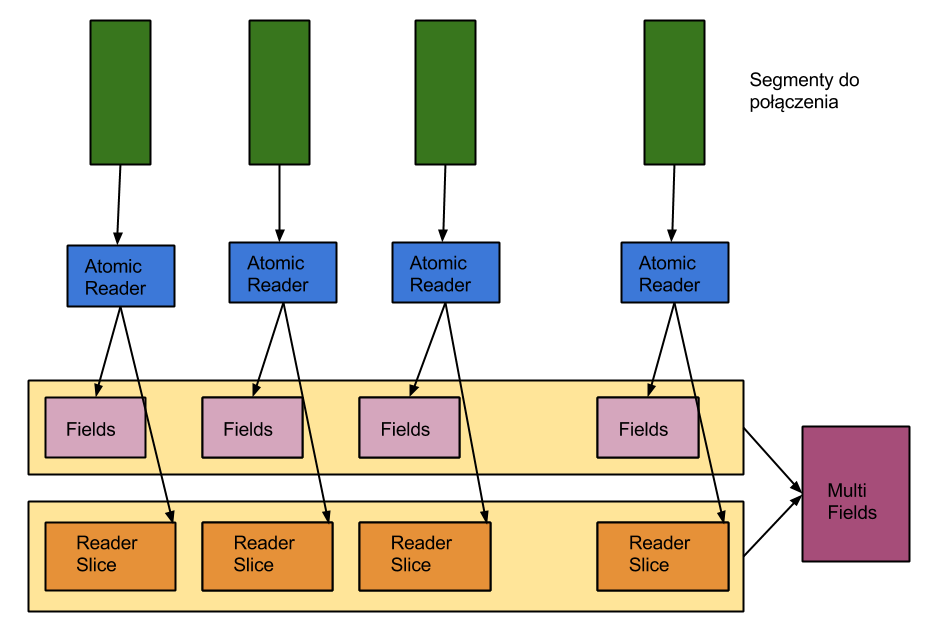
\includegraphics[scale=0.4]{pictures/LaczeniePol.png}
 \caption{Schematyczne ujęcie procesu łączenia pól z różnych segmentów. Źródło: opracowanie własne. \label{fig:fieldMerge}}
\end{figure}

\section{\texttt{MultiFields}}

W procesie łączenia list postingowych mamy do czynienia ze specyficznymi rozszerzeniami klas \texttt{Fields}, \texttt{Terms} i \texttt{DocsEnum}. Są to \texttt{MultiFields}, \texttt{MultiTerms} oraz \texttt{MultiDocsEnum} i jej pochodne. Stanowią one agregatory wielu instancji, odpowiednio, \texttt{Fields}, \texttt{Terms}, \texttt{DocsEnum} i ich zadaniem jest takie operowanie tymi wewnętrznymi instancjami, aby inne klasy ,,nie wiedziały'' że mają do czynienia z agregatem. Innymi słowy, klasy \texttt{MultiX} przedstawiają zbiór swoich instancji \texttt{X} w taki sposób, jakby był to pojedynczy obiekt typu \texttt{X}. \texttt{MultiX} dziedziczy zatem interfejs (zachowanie) klasy \texttt{X} (gdzie \texttt{X} oznacza, odpowiednio, \texttt{Fields}, \texttt{Terms} lub \texttt{DocsEnum}).

\texttt{MultiFields} jest najbardziej złożoną z takich klas. Zgodnie z tym, co zostało powiedziane w poprzednim akapicie, jest ona rozszerzeniem klasy \texttt{Fields}. Ponadto grupuje w sobie reprezentacje pól pochodzących z różnych segmentów i pozwala na operowanie ich zawartością tak, jakby były to pola pobrane z jednego segmentu. Jej schemat (oraz schematy klas powiązanych) przedstawia rys. \ref{multiFields}.

\begin{figure}[here]
 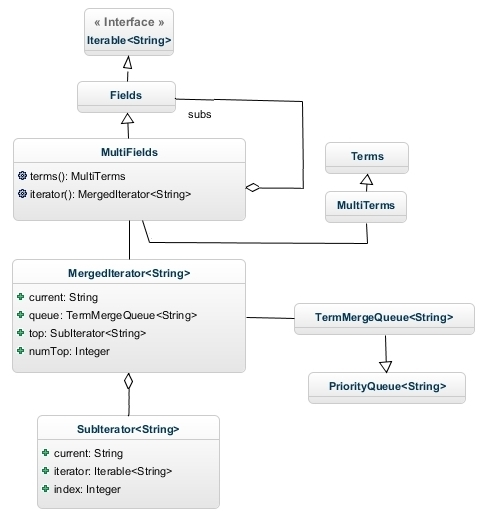
\includegraphics[scale=0.65]{pictures/MultiFields_2.jpg}
 \caption{\texttt{MultiFields} oraz klasy powiązane. Źródło: opracowanie własne.\label{multiFields}}
\end{figure}

To, że \texttt{MultiFields} jest rozszerzeniem klasy \texttt{Fields} oznacza, że posiada wszystkie jej funkcjonalności i w ich obrębie posługuje się takim samym interfejsem. Z punktu widzenia klasy zarządzającej procesem łączenia segmentów (\texttt{SegmentMergera}) zachowuje się więc dokładnie jak \texttt{Fields} (o tym właśnie była mowa w pierwszym akapicie tej sekcji). Jest to przykład dobrego podziału odpowiedzialności pomiędzy klasami i ukrywania wewnętrznej implementacji.

Z punktu widzenia algorytmu łączenia segmentów, najbardziej interesującymi metodami \texttt{MultiFields} są \texttt{MultiFields.terms(String field)}, zwracająca termy należące do pola o podanej nazwie oraz \texttt{MultiFields.iterator()}, zwracająca iterator pozwalający na przechodzenie po kolejnych nazwach pól. Bowiem gdy definicje pól zostaną już połączone (co odbyło się poprzez utworzenie instancji \texttt{MultiFields}), w ramach każdego z nich zostaną połączone termy. A termy dla danego pola o nazwie \texttt{fieldName} one zostaną zwrócone właśnie przez \texttt{MultiFields.terms(String fieldName)}.

\section{\texttt{MultiFields.terms()}}

\texttt{MultiFields.terms()} zwraca instancję typu \texttt{MultiTerms}. Podobnie jak \texttt{MultiFields} agreguje pola z różnych segmentów, ale zachowuje się tak, jak \texttt{Fields} pochodzące z pojedynczego segmentu, tak \texttt{MultiTerms}  gromadzi wszystkie termy znajdujące się w danym polu. Ukrywa też to, że dla danego termu być może mamy do czynienia z kilkoma termami o takim samym tokenie, ale pochodzącymi z tego samego pola z różnych segmentów.

Schemat tworzenia instancji \texttt{MultiTerms} znajduje się na rys. \ref{fig:multiTerms}. Nietrudno dostrzec podobieństwo z algorytmem tworzenia instancji \texttt{MultiFields} (rys. \ref{fig:fieldMerge}). Instancje \texttt{Terms} są pobrane przy pomocy \texttt{Fields.terms(f)} dla \texttt{f} będącego nazwą pola przechowywanego przez \texttt{MultiFields}. Jeśli obiekt \texttt{Terms} istnieje dla danego pola (tzn. \texttt{terms(f) != null}), podawany jest, wraz z odpowiadającym mu obiektem \texttt{ReaderSlice}, do właśnie tworzonej instancji \texttt{MultiTerms}.

\begin{figure}[here]
 \centering
 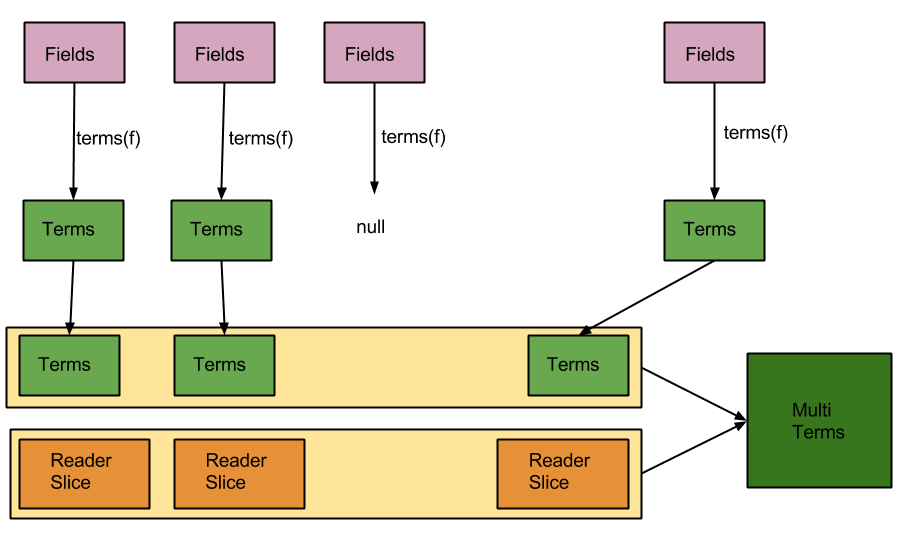
\includegraphics[scale=0.4]{pictures/MultiTerms.png}
 \caption{Schemat tworzenia instancji \texttt{MultiTerms}. Źródło: opracowanie własne. \label{fig:multiTerms}}
\end{figure}

\section{\texttt{MultiFields.iterator()}}

Jak zostało to już wspomniane, \texttt{Fields.iterator()} przechodzi po nazwach pól zgromadzonych w klasie \texttt{Fields}. Kolejne elementy zwracane przez ten iterator są uporządkowane rosnąco. \texttt{MultiFields.iterator()}, aby spełnić to wymaganie, posługuje się własną implementacją iteratora napisów -- klasą \texttt{MergedIterator}. Oto jej specyfikacja:
\begin{itemize}
 \item \texttt{MergedIterator} jest tworzony na podstawie iteratorów napisów $i_1$, $i_2$, ... $i_n$. Zwraca kolejno elementy tych iteratorów posortowane rosnąco; 
 \item jeśli dany element występuje w więcej niż jednym z iteratorów $i_1$, $i_2$, ... $i_n$, \texttt{MergedIterator} zwraca go tylko raz.
\end{itemize}
Iteratory $i_1$, $i_2$, ... $i_n$ pochodzą z instancji \texttt{Fields} zgromadzonych w \texttt{MultiFields}. \texttt{MergedIterator} wykorzystuje kolejkę priorytetową do przechowywania zagregowanych iteratorów. Porządek kolejki jest zdefiniowany przez elementy, na które w danym momencie wskazują iteratory $i_k, k \in \{1, ..., n\}$.

\section{Łączenie termów}
\label{sec:termsMerge}

Łączenie termów odbywa się w metodzie \texttt{merge()} klasy \texttt{TermsConsumer}, która jako parametry przyjmuje:
\begin{itemize}
 \item \texttt{MergeState} -- pomocniczy obiekt przechowujący stan obecnego procesu łączenia segmentów. Gromadzi listę \texttt{AtomicReaderów}, strukturę z informacją o dokumentach do usunięcia, itp;
 \item \texttt{IndexOptions} -- wartość wskazująca na to, jakie informacje o termach i ich wystąpieniach zostały zaindeksowane. \texttt{IndexOptions} przyjmuje jedną z czterech wartości:
 \begin{enumerate}
  \item \texttt{DOCS\_ONLY}: oznacza, że w indeksie znajduje się tylko informacja o tym, czy dany term tam wystąpił, czy nie. Częstości występowania termu oraz pozycje wystąpień są pominięte -- co skutkuje np. tym, że zapytania frazowe nie mogą zostać na takim indeksie wykonane. Obliczanie zgodności zapytania z dokumentem zachowuje się tak, jakby każdy term występował w dokumencie dokładnie raz.
  \item \texttt{DOCS\_AND\_FREQS}: dla każdego termu zapamiętana jest informacja o jego liczbie wystąpień w dokumencie. Dzięki temu podobieństwo zapytania do dokumentu może być obliczone precyzyjniej. Zapytania frazowe oraz inne, wykorzystujące informacje o pozycjach termów, nie mogą być wykonywane.
  \item \texttt{DOCS\_AND\_FREQS\_AND\_POSITIONS}: najczęściej wykorzystywany sposób indeksowania: w indeksie pamiętane są częstości termów oraz pozycje ich wystąpień, w związku z czym możliwe jest wykonywanie wielu typów zapytań.
  \item \texttt{DOCS\_AND\_FREQS\_AND\_POSITIONS\_AND\_OFFSETS}: poza częstościami i pozycjami wystąpień termów pamiętane są informacje o dokładnym położeniu każdego termu (tzn. odległości znakowej od początku dokumentu) i jego faktycznej długości (pamiętamy o tym, że różne formy danego termu podczas analizy są sprowadzane do formy bazowej -- dlatego informacja o pierwotnej długości wystąpienia musi być dodatkowo zapamiętana).
 \end{enumerate}
 \item \texttt{TermsEnum} -- w procesie łączenia termów będzie to instancja \texttt{MultiTermsEnum}, pobrana z obiektu \texttt{MultiTerms}.
\end{itemize}

Jak pamiętamy, łączenie termów natępuje w ramach jednego (dopiero co połączonego) pola \texttt{f}, zawartego w obiekcie typu \texttt{MultiFields}. Aby termy zostały połączone, instancja ta musi wylistować wszystkie termy należące do \texttt{f}. Poprzez wywołanie \texttt{MultiFields.terms(s)} tworzy więc dla \texttt{f} obiekt typu \texttt{MultiTerms}, z którego z kolei jest pobrana instancja iteratora termów -- \texttt{MultiTermsEnum} (konkretniej: \texttt{MultiTermsEnum} jest wynikiem wywołania \texttt{MultiTerms.iterator()}). Właśnie ona będzie odgrywała najważniejszą rolę w dalszej części procesu.

W najprostszym przypadku -- dla opcji \texttt{DOCS\_ONLY} -- algorytm łączenia termów wygląda następująco:
\begin{enumerate}
 \item Zainicjalizuj \texttt{visitedDocs} -- zbiór dokumentów odwiedzonych już dla właśnie łączonego pola.
 \item Zainicjalizuj pole \texttt{docsEnum} typu \texttt{MappingMultiDocsEnum}, o ile nie zostało to jeszcze zrobione (leniwa inicjalizacja -- właśnie łączony term jest pierwszym z termów pola).
 \item Dla każdego termu \texttt{t} dostępnego z \texttt{MultiTermsEnum} pobierz listę \texttt{docsEnumIn} dokumentów, w których term ten występuje. Lista opakowana jest w instancję klasy \texttt{MultiDocsEnum}. Dodaj dokumenty z \texttt{docsEnumIn} do \texttt{docsEnum}. Wykonaj kroki \ref{enum:begin} -- \ref{enum:end} dla \texttt{t}.
 \item \label{enum:begin} Rozpocznij zapis listy postingowej dla \texttt{t} (przy pomocy wywołania \texttt{startTerm(t)}). Jednocześnie pobierz instancję \texttt{PostingsConsumera}, która umożliwi połączenie list postingowych pochodzących z różnych segmentów.
 \item \label{alg:postingsConsumerMergeCall} Wywołaj \texttt{PostingsConsumer.merge()}, jako parametry przekazując obiekt przechowujący stan (\texttt{MergeState}), \texttt{DOCS\_ONLY} jako opcję indeksowania, \texttt{docsEnum} i listę odwiedzonych już dokumentów \texttt{visitedDocs}.
 \item \label{enum:end} Zakończ zapis termu (\texttt{PostingsConsumer.finishTerm()}), zapamiętaj liczbę dokumentów w połączonej liście.
 \item Zakończ algorytm.
\end{enumerate}

Dla pozostałych wartości parametru \texttt{IndexOptions} łączenie termów przebiega podobnie. Różni się jedynie typami struktur przechowujących referencje do list postingowych.
\begin{itemize}
 \item W przypadku \texttt{DOCS\_AND\_FREQS} korzystamy z innej instancji typu \\ \texttt{MappingMultiDocsEnum} -- \texttt{docsAndFreqsEnum}, zamiast \texttt{docsEnum}.
 \item W przypadkach \texttt{DOCS\_AND\_FREQS\_AND\_POSITIONS} oraz \\ \texttt{DOCS\_AND\_FREQS\_AND\_POSITIONS\_AND\_OFFSETS} korzystamy z tej samej instancji klasy \texttt{MappingMultiDocsAndPositionsEnum}, \texttt{postingsEnum}.
\end{itemize}
Różne typy i różne instancje przechowujące dane o listach postingowych są tutaj potrzebne, ponieważ w ramach jednego procesu łączenia segmentów możemy mieć do czynienia z różnymi opcjami indeksowania pól (jak już wspomniano, opcje indeksowania pól są całkowicie od siebie niezależne, nawet dla pól występujących w tym samym segmencie).

\section{Łączenie list postingowych}

Łączenie list postingowych jest zaimplementowane w metodzie \texttt{merge()} klasy \texttt{PostingsConsumer} (por. krok \ref{alg:postingsConsumerMergeCall} algorytmu w sekcji \ref{sec:termsMerge}). Metoda ta przyjmuje następujące parametry, przekazywane z \texttt{TermsConsumer.merge()}:
\begin{itemize}
 \item \texttt{MergeState}: przekazany bez zmian z instancji \texttt{TermsConsumera}. Przydatny będzie do uzyskania informacji o dokumentach usuniętych.
 \item \texttt{IndexOptions}: podobnie, jak w przypadku łączenia termów, dokładny algorytm zależy od wybranej opcji indeksowania.
 \item \texttt{DocsEnum}: reprezentacja list dokumentów, które mają być połączone. Obecny kodek wykorzystuje \texttt{MappingMultiDocsEnum} lub \\ \texttt{MappingMultiDocsAndPositionsEnum}, w zależności od opcji indeksowania (i instancji przekazanej tutaj z \texttt{TermsConsumer.merge()}). 
 \item \texttt{FixedBitSet}: zbiór bitowy reprezentujący odwiedzone już dokumenty (\texttt{visitedDocs} z algorytmu w sekcji \ref{sec:termsMerge}).
\end{itemize}

Podobnie jak w \texttt{TermsConsumer.merge()}, opcje indeksowania wpływają na algorytm łączenia list. W najprostszym przypadku (dla \texttt{IndexOptions.DOCS\_ONLY}) algorytm ten ma następujący przebieg:
\begin{enumerate}
 \item \label{jeden} Pobierz kolejny posting z listy (z \texttt{DocsEnum}) do zmiennej \texttt{doc}. Jeśli otrzymaną wartością jest \texttt{NO\_MORE\_DOCS}, zakończ algorytm. W przeciwnym wypadku przejdź do kroku \ref{dwa}.
 \item \label{dwa} Zaznacz \texttt{doc} jako odwiedzony (skorzystaj z dostarczonej instancji \texttt{FixedBitSet}).
 \item \label{trzy} Rozpocznij zapis postingu. Zapisz wartość \texttt{doc} do listy wynikowej.
 \item Zakończ zapis postingu.
 \item Przejdź do kroku \ref{jeden}.
\end{enumerate}

W przypadku innych opcji indeksowania do powyższego algorytmu wprowadza się kilka zmian.
\begin{itemize}
 \item Dla opcji \texttt{DOCS\_AND\_FREQS}, poza pobraniem postingu z listy \texttt{DocEnum} w kroku \ref{jeden}, odczytuje się także częstość występowania termu w dokumencie, \texttt{docFreq}, która później zapisywana jest wraz z postingiem w kroku \ref{trzy}.
 \item Dla opcji \texttt{DOCS\_AND\_FREQS\_AND\_POSITIONS} dodatkowo odczytywane są (i później zapisywane do listy wynikowej) pozycje wystąpień termu w dokumencie oraz ewentualne \emph{payloads}, a dla \texttt{DOCS\_AND\_FREQS\_AND\_POSITIONS\_AND\_OFFSETS} -- również ich odległości znakowe od początku dokumentu i długości. Wszystkie te informacje zapisywane są wraz z postingiem w kroku \ref{trzy}.
\end{itemize}

\section{Rozszerzenia klasy \texttt{DocsEnum} używane w procesie łączenia postingów}

\texttt{DocsEnum} jest abstrakcją pozwalającą pobierać kolejne elementy list postingowych. Jej interfejs zawiera jedynie metody zwracające numer dokumentu obecnie wskazywanego przez iterator, jego częstość oraz pozwalające na przejście do kolejnych dokumentu. Dodatkowe funkcjonalności są implementowane przez jej liczne rozszerzenia (np. wspomniany już \texttt{DocsAndPostitionsEnum}). W algorytmie łączenia list postingowych wykorzystywane są cztery z nich: \texttt{MultiDocsEnum}, \texttt{MappingMultiDocsEnum} oraz odpowiadające im \texttt{MultiDocsAndPositionsEnum} i \texttt{MappingMultiDocsAndPositionsEnum}. Przyjrzymy się im dokładniej.

Podczas łączenia termów (w metodzie \texttt{TermsConsumer.merge()}) z iteratora termów (konkretniej: z instancji \texttt{MultiTermsEnum}) pobierany jest obiekt \texttt{MultiDocsEnum}. Zawiera on informacje o listach postingowych dla danego termu pochodzących z łączonych segmentów oraz odpowiadające im wskaźniki na dany segment (w postaci obiektów \texttt{ReaderSlice}). Schemat klasy \texttt{MultiDocsEnum} przedstawia rys. \ref{fig:multiDocsEnum}.

\begin{figure}[here]
 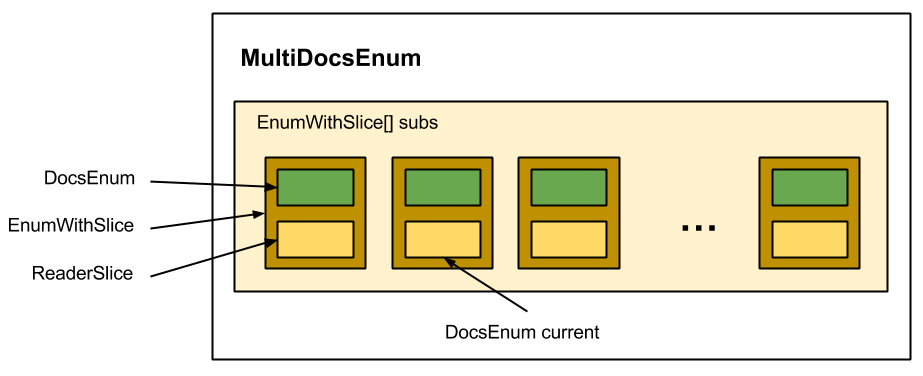
\includegraphics[scale=0.4]{pictures/MultiDocsEnum.png}
 \caption{\texttt{MultiDocsEnum} i jej zawartość. Źródło: opracowanie własne. \label{fig:multiDocsEnum}}
\end{figure}

Poza innymi wskaźnikami i zmiennymi, \texttt{MultiDocsEnum} posługuje się zmienną \texttt{current} wskazującą na obecnie odczytywany iterator dokumentów -- \texttt{current} odwiedza wszystkie zgromadzone obiekty \texttt{DocsEnum} i iteruje po ich zawartości. Przeskakuje na następny w momencie wyczerpania postingów w obecnie odwiedzanej instancji \texttt{DocsEnum}. Dzięki temu, z punktu widzenia klasy \texttt{PostingsConsumer}, \texttt{MultiDocsEnum} zachowuje się dokładnie tak samo, jak każdy \texttt{DocsEnum} -- pomimo, że faktycznie jest agregatem obiektów typu \texttt{DocsEnum}. 

Obiekty \texttt{ReaderSlice} służą z kolei do odczytywania podstawy przenumerowania dokumentów pochodzących z danego segmentu.

\texttt{MappingMultiDocsEnum}, poza wymienionymi wyżej strukturami, zawiera także infomację o tym, które dokumenty powinny zostać usunięte podczas łączenia segmentów. Jest ona przechowywana w strukturze \texttt{DocMap} i pobierana jest z instancji \texttt{MergeState} (rys. \ref{fig:mappingMultiDocsEnum}). Instancja \texttt{MappingMultiDocsEnum} jest tworzona podczas łączenia termów w metodzie \texttt{TermsConsumer.merge()} -- listy postingowe z pobranego wcześniej obiektu \texttt{MultiDocsEnum} są do niej kopiowane i w dalszej części algorytmu wszystkie operacje na tych listach wykonywane są właśnie na kopiach znajdujących się w \texttt{MappingMultiDocsEnum}. 

Celem tego zabiegu jest zachowanie podzielonej odpowiedzialności: zadaniem \texttt{MultiDocsEnum} jest gromadzenie kilku \texttt{DocsEnum} i przedstawianie ich w postaci jednego iteratora. \texttt{MappingMultiDocsEnum} natomiast do tych funkcjonalności dodaje jeszcze możliwość pomijania dokumentów gotowych do usunięcia z indeksu. 

\begin{figure}[here]
 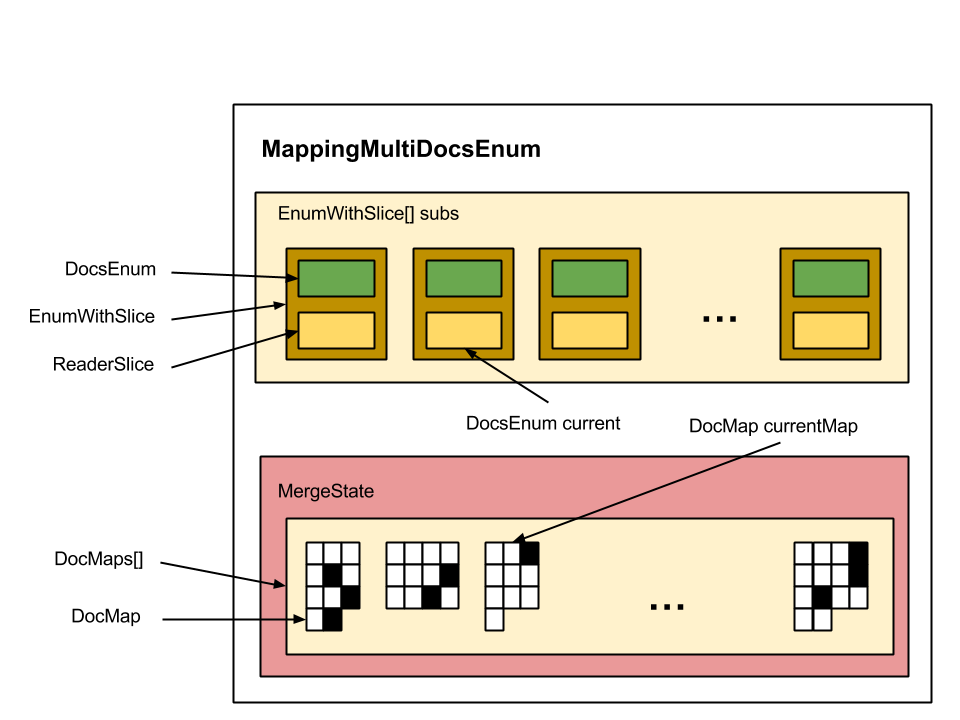
\includegraphics[scale=0.4]{pictures/MappingMultiDocsEnum.png}
 \caption{\texttt{MappingMultiDocsEnum}. Źródło: opracowanie własne. \label{fig:mappingMultiDocsEnum}}
\end{figure}

Gdy \texttt{MappingMultiDocsEnum} pytany jest o kolejny dokument z właśnie rozpatrywanej listy postingowej, sprawdza najpierw w odpowiedniej instancji \texttt{DocMap}, czy kolejny wskazywany dokument na liście jest ,,żywy''. Podaje jego numer tylko wtedy, jeśli faktycznie tak jest. W ten sposób dokumenty zaznaczone do usunięcia są pomijane w procesie łączenia list. 

Przepisywanie zawartości jednej klasy do drugiej nie jest najelegantszym rozwiązaniem -- z punktu widzenia czystości kodu lepsze byłoby tutaj zastosowanie wzorca projektowego \emph{dekorator}: \texttt{MappingMultiDocsEnum} mógłby opakowywać instancję \texttt{MultiDocsEnum} i jednocześnie rozszerzać funkcjonalność \texttt{DocsEnum} o pomijanie dokumentów gotowych do usunięcia.

\section{Propozycja optymalizacji algorytmu łączenia list postingowych}

\subsection{Opis problemu}

Zauważmy, że w procesie łączenia list postingowych numery dokumentów przepisywane są pojedynczo: dowolne rozszerzenie \texttt{DocsEnum} potrafi podawać kolejne postingi, jeden za drugim, bez możliwości ich grupowania. Listy postingowe w plikach indeksu trzymane są w formie zakodowanej (por. \ref{sec:packedBlockEncoding} i \ref{sec:vIntEncoding}), natomiast numery dokumentów gotowych do usunięcia są (w uproszczeniu) dostępne jako liczby całkowite. W związku z tym, podczas łączenia list postingowych każdy posting musi być odkodowany w celu sprawdzenia, czy ma on być zapisany do listy wynikowej, czy nie. Jeśli dany dokument jest ,,żywy'' (nie znajduje się na liście dokumentów do usunięcia), jego numer musi zostać ponownie zakodowany przed zapisaniem. Zatem dla list postingowych długości $l_1$ i $l_2$ wykonujemy $O(l_1 + l_2)$ operacji odkodowania i zakodowania liczby całkowitej.

W większości systemów wyszukiwania dokumenty usuwane są dość rzadko -- co oznacza, że w ogólnym przypadku liczba ,,martwych'' postingów w łączonych listach jest stosunkowo mała. W związku z tym często możnaby unikać niepotrzebnych operacji kodowania i odkodowania. Wymaga to jednak modyfikacji algorytmu łączenia list: chcielibyśmy móc niekiedy kopiować całe zakodowane bloki zamiast pojedynyczych postingów. Pomysł taki został zgłoszony w systemie zarządzania zadaniami związanym z Lucene (Lucene Jira, \cite{jira}). Jego skrótowy opis znajduje się w \cite{idea}.

Blok postingów mógłby zostać przekopiowany bez dekodowania, o ile liczba dokumentów usuniętych znajdujących się w nim byłaby stosunkowo mała (implementacja rozwiązania zawierałaby modyfikowalną maksymalną dopuszczalną liczbę ,,martwych'' dokumentów w bloku). Jeśli w danym bloku byłoby więcej dokumentów do usunięcia, byłby on przepisywany tak, jak dotychczas -- po jednym elemencie.

\subsection{Proponowane rozwiązanie}
\label{sec:solution}

W tej sekcji omówione zostanie proponowane rozwiązanie dla najprostszego przypadku indeksowania (\texttt{IndexOptions.DOCS\_ONLY}). Wprowadzenie opisanej wyżej modyfikacji wymaga rozwiązania dwóch problemów:
\begin{enumerate}
 \item w jaki sposób zmienić architekturę części odpowiadającej za łączenie list postingowych tak, aby istniała możliwość kopiowania zarówno bloków (bez dekodowania) oraz pojedynczych postingów?
 \item jak wyznaczyć bloki gotowe do przekopiowania?
\end{enumerate}

Zmiany w architekturze rozpoczynają się od wprowadzenia klasy reprezentującej element listy postingowej, \texttt{PostingElement}. Jej schemat specyfikuje rys. \ref{fig:postingElement}. W zależności od tego, jaki fragment listy postingowej jest zwracany (\texttt{type} przyjmujące wartość \texttt{PostingElementType.BLOCK} lub \texttt{PostingElementType.INT}), inicjalizowane jest pole \texttt{postingBlocks} lub \texttt{posting}.

\begin{figure}[here]
 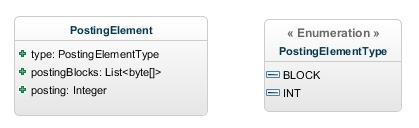
\includegraphics[scale=0.7]{pictures/PostingElement.jpg}
 \caption{Klasa \texttt{PostingElement}. Źródło: opracowanie własne. \label{fig:postingElement}}
\end{figure}

Dodatkowo, potrzebne są też odpowiedniki klas \texttt{DocsEnum} oraz \texttt{MultiDocsEnum} potrafiące się nią posługiwać. Wprowadzamy więc \texttt{PostingElementEnum} oraz \texttt{MultiPostingElementEnum} (rys. \ref{fig:postingEnums}).

\begin{figure}[here]
 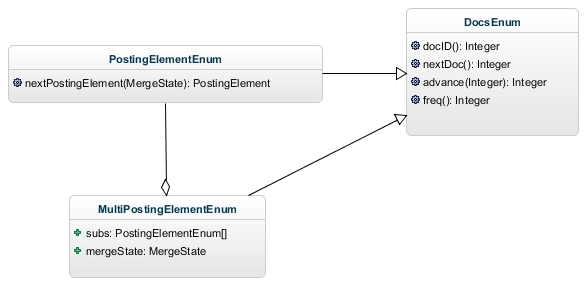
\includegraphics[scale=0.7]{pictures/PostingEnums.jpg}
 \caption{\texttt{PostingElementEnum} oraz \texttt{MultiPostingElementEnum} -- rozszerzenia \texttt{DocsEnum} wykorzystywane w zmodyfikowanym algorytmie łączenia list postingowych. Źródło: opracowanie własne. \label{fig:postingEnums}}
\end{figure}

Taka zmiana wymaga uzasadnienia kilku kwestii.
\begin{enumerate}
 \item \label{item:inheritance} Jak można odczytać z diagramu \ref{fig:postingEnums}, zarówno \texttt{PostingElementEnum} oraz \texttt{MultiDocsAndPositionsEnum} rozszerzają klasę \texttt{DocsEnum} i w związku z tym dziedziczą jej interfejs, posługujący się jedynie liczbami całkowitymi. Na pierwszy rzut oka może to wydawać się niezgodne z ideą zmiany -- chcemy wszak wprowadzić abstrakcję opakowującą elementy list postingowych (do tego służy nam właśnie \texttt{PostingElement}) i nowe klasy powinny się tylko nią posługiwać. Dziedziczenie po \texttt{DocsEnum} służy tutaj zachowaniu zgodności z resztą systemu. Chcemy, aby wprowadzone zmiany w jak najmniejszym stopniu modyfikowały istniejący interfejs programisty biblioteki i jak najmniej ingerowały w strukturę klas -- w szczególności, jeśli nie są to klasy pojedynczego kodeka, a klasy wspólne, wykorzystywane przez wszystkie kodeki. Dodatkowo, dziedziczenie po \texttt{DocsEnum} pozwoli nam wykorzystać to, że lista postingowa jest skip listą (co okaże się przydatne podczas wyznaczania fragmentu listy do późniejszego przekopiowania).
 \item Wszystkie metody klasy \texttt{DocsEnum} są abstrakcyjne. W związku z tym, dużo bardziej elegancko byłoby posłużyć się w tym wypadku interfejsem (najlepiej parametryzowanym), a nie klasą abstrakcyjną. Możnaby wtedy uprościć hierarchię iteratorów postingów dzięki wykorzystaniu wielodziedziczenia (w Javie klasy mogą dziedziczyć tylko po jednej klasie bazowej -- mogą natomiast implementować wiele interfejsów): funkcjonalność iterowania po postingach można byłoby wtedy oddzielić od funkcjonalności grupowania innych iteratorów. Taka zmiana wymagałaby jednak przebudowania znacznej części Lucene. Warto wspomnieć to, że \texttt{DocsEnum} dziedziczy implementację metody \texttt{slowAdvance(int target)} po \texttt{DocIdSetIteratorze}. Zatem przepisanie abstrakcyjnego \texttt{DocsEnum} na interfejs wymagałoby przeniesienia implementacji \texttt{slowAdvance()} w inne miejsce. Ponadto, zmiany tego typu prawdopodobnie nie poprawiłyby niczego poza czytelnością kodu. Praktycznie rzecz biorąc nie warto więc ich wprowadzać.
 \item W punkcie \ref{item:inheritance} jako jeden z argumentów za dziedziczeniem \texttt{PostingElementEnum} z \texttt{DocsEnum} wspomniane zostało współdzielenie operowania na liście postingowej jak na skip liście. Możnaby tutaj pokusić się o oddzielenie tego zadania od reszty funkcjonalności \texttt{DocsEnum} poprzez wyekstrahowanie interfejsu \texttt{Skippable}, gromadzącego metody \texttt{advance(int target)} i \texttt{slowAdvance(int target)}. Poprzez wprowadzenie relacji implementowania interfejsu pomiędzy \texttt{DocsEnum} i \texttt{Skippable} oraz \texttt{PostingElementEnum} i \texttt{Skippable}, zależność między \texttt{DocsEnum} i \texttt{PostingElementEnum} byłaby rozluźniona -- potencjalnie możnaby nawet zrezygnować z relacji dziedziczenia pomiędzy tymi klasami. Wadą takiego rozwiązania byłby brak możliwości dziedziczenia implementacji metody \texttt{slowAdvance()}, która w obecnym kształcie systemu jest taka sama dla wszystkich iteratorów elementów list postingowych.
\end{enumerate}

Wprowadzenie \texttt{PostingElement} oraz nowych iteratorów postingów wymaga też zmian w metodach \texttt{merge()} klas \texttt{TermsConsumer} oraz \texttt{PostingsConsumer}. Iterowanie po postingach i ich odczyt jest wykonywany przez \texttt{PostingElementEnum}, samo łączenie odbywa się w metodzie wspomnianej powyżej. Dodatkowo, \texttt{Postings}-\texttt{Consumer} (a dokładniej: jego rozszerzenie przypisane do danego kodeka) jest odpowiedzialny za zapis list postingowych. Należy zatem dodać mu funkcjonalność zapisu zakodowanych bloków postingów. 

Od strony implementacyjnej, najprostszym sposobem dodania wspomnianych funkcjonalności jest zastosowanie wzorca projektowego \emph{dekorator}: opakowanie klasy \texttt{PostingsConsumer} w klasę, która jednocześnie dziedziczyć będzie po niej zachowanie. Klasę opakowującą nazwijmy \texttt{BlockPostingsConsumer}. Jej nowe funkcjonalności są zaimplementowane bezpośrednio, natomiast fukcjonalności dziedziczone z \texttt{PostingsConsumer} są delegowane do wewnętrznej instancji tego typu. Metoda \texttt{merge()}, pochodząca z \texttt{PostingsConsumer} jest nadpisana w \texttt{BlockPostingsConsumer}.

\begin{figure}[here]
 \centering
 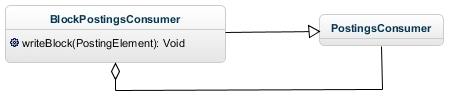
\includegraphics[scale=0.8]{pictures/PostingsConsumerWrapper.jpg}
 \caption{\texttt{BlockPostingsConsumer} -- dekorator dla \texttt{PostingsConsumera}. Źródło: opracowanie własne. \label{fig:postingsConsumerWrapper}}
\end{figure}

Samo utworzenie instancji \texttt{BlockPostingsConsumer} mogłoby się odbywać w \texttt{TermsConsumer.merge()}. Instancja odpowiedniego dla kodeka \texttt{PostingsConsumera} zaraz po pobraniu byłaby opakowywana w nowe funkcjonalności poprzez wstrzyknięcie jej do konstruktora klasy \texttt{BlockPostingsConsumer}.

Ponadto, w klasie \texttt{TermsConsumer} pole \texttt{docsEnum} powinno zmienić typ z \texttt{MappingMultiDocsEnum} na \texttt{MultiPostingElementEnum}.

Nowy algorytm łączenia termów (\texttt{TermsConsumer.merge()}), wykorzystujący wyżej opisane zmiany, wyglądałby więc następująco:
\begin{enumerate}
 \item Zainicjalizuj pole \texttt{docsEnum} typu \texttt{MultiPostingElementEnum}, o ile nie zostało to jeszcze zrobione.
 \item Dla każdego termu \texttt{t} dostępnego z \texttt{MultiTermsEnum} pobierz iterator \texttt{docsEnumIn} typu \texttt{MultiPostingElementEnum} (ponieważ podczas łączenia termów mamy listy postingowe pochodzące z różnych segmentów, wiemy, że pobrany iterator jest agregatorem innych iteratorów).
 \item Rozpocznij zapis listy postingowej dla \texttt{t} (przy pomocy wywołania \texttt{startTerm(t)}). Pobierz instancję \texttt{PostingsConsumera}, i podaj ją jako parametr konstruktora klasy \texttt{BlockPostingsConsumer}.
 \item Wywołaj \texttt{BlockPostingsConsumer.merge()} z odpowiednimi parametrami (instancją \texttt{MergeState}, flagą opcji indeksowania oraz zmienną \texttt{docsEnumIn}).
 \item Zakończ zapis termu (\texttt{BlockPostingsConsumer.finishTerm()}).
\end{enumerate}

Jak widać, za łączenie postingów jest teraz odpowiedzialna klasa \texttt{BlockPostingsConsumer}. Oto szkic algorytmu łączenia list, do zaimplementowania w \texttt{BlockPostingsConsumer.merge()}. Metoda ta powinna przyjmować następujące parametry: \texttt{MergeState mergeState}, \texttt{IndexOptions indexOptions} i \texttt{PostingElementEnum postingsElementEnum}.
\begin{enumerate}
 \item Tak długo jak \texttt{postingsElementEnum} jest niepusty, wykonuj kroki \ref{newMergeBegin} -- \ref{newMergeEnd}.
 \item \label{newMergeBegin} Do zmiennej \texttt{posting} pobierz kolejny \texttt{PostingElement} z \texttt{postingsElementEnum}.
 \item \label{newMergeEnd} Jeśli \texttt{posting} jest typu \texttt{PostingElementType.BLOCK}, zapisz cały blok (lub bloki) przy pomocy \texttt{BlockPostingsConsumer.writeBlocks(posting.getBlocks())}. Jeśli \texttt{posting} jest typu \texttt{PostingElementType.INT}, skorzystaj ze ,,starego'' sposobu zapisu pojedynczego postingu (\texttt{PostingsConsumer.startTerm()}, \texttt{PostingsConsumer.finishTerm()}).
 \item Zakończ algorytm.
\end{enumerate}

Do rozwiązania pozostaje jeszcze następująca kwestia: jak ustalić, który fragment listy postingowej (pojedyncza wartość, pojedynczy blok, wiele bloków) powinien zostać przekopiowany? Klasą, która powinna o tym decydować będzie \texttt{PostingElementEnum} lub klasa z niej wywiedziona. 

Pomimo, że wszystkie bloki list postignowych są zakodowane i nie możemy pobrać z nich wartości bezpośrednio, możemy wykorzystać tzw. \texttt{skipData}. Pamiętamy, że lista postingowa jest skip listą. Przed każdym blokiem postingów zapisywana jest informacja o wskaźnikach do tego bloku oraz (odkodowana) wartość pierwszego elementu bloku. Mając dany \texttt{mergeState}, potrafimy wylistować numery wszystkich dokumentów usuniętych. Możemy więc ustalić (posługując się skip listą), o jak wiele bloków odległy jest kolejny element usunięty i bloki bez usunięć przekopiować bez dekodowania.

Jeśli okazałoby się, że w obecnym bloku występują dokumenty usunięte, możemy ustalić ich liczbę -- i na tej podstawie zdecydować, czy blok powinien być przekopiowany w całości, czy po jednym elemencie. 

Te obliczenia wykonywać powinna metoda \texttt{PostingElementEnum.nextPostingElement()}. Jak widać na diagramie \ref{fig:postingEnums}, przyjmuje ona jako parametr obiekt typu \texttt{MergeState} -- ponieważ to właśnie ten obiekt stanu umożliwia odczytanie listy dokumentów usuniętych.

\subsection{Potencjalne problemy i uwagi dotyczące zaproponowanego rozwiązania}

Sekcja \ref{sec:solution} opisuje wysokopoziomową koncepcję rozwiązania -- jedyne, co pozostaje do zrobienia to przekucie jej na kod. Należy jednak pamiętać o tym, że wiele drobnych problemów może się ujawnić także na etapie implementacji. Poniżej naszkicowanych zostanie kilka kwestii tego typu. To, czy faktycznie okażą się one trudnością, pozostaje do zweryfikowania podczas pracy nad kodem, na etapie testowania lub nawet w trakcie działania systemu. 
\begin{enumerate}
 \item Jak zostało to niejednokrotnie wspomniane, dokumenty numerowane są od zera w obrębie każdego segmentu. Podczas łączenia list postingowych owe numery porządkowe są zmieniane poprzez dodanie do nich tzw. bazy, która obliczana jest jako łączna liczba dokumentów w listach już połączonych. Zatem, aby poprawnie zapisywać numery dokumentów w sytuacji, w której pierwszy blok listy będzie przekopiowany bez dekodowania, tak czy inaczej należy odkodować pierwszy posting tego bloku, dodać do niego bazę oraz obliczyć różnicę pomiędzy wartością tak otrzymaną a ostatnim zapisanym numerem dokumentu (pamiętamy, że na listach postingowych przechowywane są różnice między numerami dokumentów). Potencjalnie więc trzeba będzie zawsze odkodowywać cały pierwszy blok listy postingowej. W sytuacji, w której dany term rzadko występuje w zbiorze dokumentów (a więc odpowiadające mu listy postingowe są krótkie, składają się z jednego bloku), optymalizacja w ogóle nie zostanie wykorzystana.
 \item Rozwiązanie zaproponowane w \ref{sec:solution} dotyczy najprostszego przypadku indeksowania: w  indeksie pamiętane są jedynie numery dokumentów, bez częstości występowania termu i dodatkowych informacji (\texttt{IndexOptions.DOCS\_ONLY}). Należy także ustalić, w jaki sposób radzić sobie z pozostałymi przypadkami. Jest to jednak problem natury czysto implementacyjnej.
 \item Zakładamy, że jeśli w danym bloku występuje mała liczba dokumentów usuniętych, to blok także jest przepisywany bez odkodowywania. Wobec tego należy opracować sposób zapisywania numerów ,,martwych'' dokumentów w nowej generacji segmentu -- do tego warto byłoby wykorzystać część kodeka zwaną \texttt{LiveDocsFormat}.
 \item \emph{Problem niezapełnionego bloku}: rozważmy następującą sytuację: podczas przepisywania długiej listy postingowej natrafiamy na blok z dużą liczbą dokumentów usuniętych (większą niż maksymalna dopuszczalna liczba ,,martwych'' dokumentów w bloku). Należy więc przepisać ten blok ,,starym'' sposobem: element po elemencie, z pominięciem niektórych wartości. Okazuje się, że w takim wypadku blok będzie krótszy niż wymagane 128 postingów (o ile nie jest to ostatni blok listy, kodowany przy pomocy formatu \texttt{vInt}) -- co spowodowałoby sytuację, w której wszystkie kolejne bloki musiałyby być przepisywane ,,po staremu'' i optymalizacja w ogóle nie zostałaby wykorzystana. Rozwiązaniem w tym wypadku byłoby ,,dopełnienie'' niepełnego bloku specjalnymi wartościami, które nie mogą występować na listach postingowych (np. zerami). W dłuższej perspektywnie mogłoby to jednak doprowadzić do stanu, w którym większość list postingowych jest ,,pusta'' -- zawiera więcej dziur niż istotnych wartości. Możemy więc 
stwierdzić, że rozwiązanie z \ref{sec:solution} sprawdzi się tylko w systemach, w których nie spodziewamy się częstego usuwania dokumentów.
\end{enumerate}
\chapter{Podsumowanie}

W poprzednich rozdziałach pracy zostały przedstawione, kolejno: funkcjonalności Lucene, jej architektura oraz algorytm łączenia list postingowych, wraz z~propozycją jego optymalizacji.

Apache Lucene jest obecnie jedną z najczęściej używanych bibliotek wyszukiwania tekstowego. O jej popularności świadczy m.in. mnogość wykorzystujących ją projektów (dokumentacja \cite{poweredBy} wspomina o prawie 300 projektach i~stronach internetowych). Dzięki zastosowaniu architektury kodekowej, format indeksu jest całkowicie oddzielony od logiki indeksowania i~wyszukiwania. Pozwala to z powodzeniem zastosować Lucene w wielu projektach komercyjnych i~ badawczych.

\begin{thebibliography}{10}
 
 \bibitem{gutenberg} Project Gutenberg, \emph{http://www.gutenberg.org/}, dostęp IX 2013
 
 \bibitem{geopart} N. Lester, A. Moffat, J. Zobel; \emph{Fast On-Line Index Construction by Geometric Partitioning}, 2005
 
 \bibitem{flexindex} U. Schindler; \emph{Heavy Committing: Flexible Indexing in Lucene 4.0}; \emph{Lucene Revolution}, 2011
 
 \bibitem{irbook} C. D. Manning, P. Raghavan, H. Sch\"{u}tze; \emph{An Introduction to Information Retrieval}; 2009
 
 \bibitem{jira} Jira związana z Apache Lucene, \emph{https://issues.apache.org/jira/browse/LUCENE}, dostęp X 2013
 
 \bibitem{idea} LUCENE-2082: Performance improvement for merging posting lists, zgłoszony przez M. Busch, \emph{http://issues.apache.org/jira/browse/LUCENE-2082}, dostęp 10.2013
 
 \bibitem{indexReader} U. Schindler; \emph{Is your IndexReader really Atomic or Slow?}; \emph{Lucene Revolution}, 2012
 
 \bibitem{liceneInAction} E. Hatcher, O. Gospodnetic, M. McCandless; \emph{Lucene in Action. Second edition}; Manning, 2009
 
 \bibitem{documentation} Dokumentacja Lucene Core, \emph{http://lucene.apache.org/core/}, dostęp X 2013
 
\end{thebibliography}


\end{document}
